\documentclass[spanish,12pt,a4paper,final,oneside]{book}
\setlength{\parindent}{0pt}
\setlength{\parskip}{0.5em}
\usepackage[spanish]{babel}
\usepackage[utf8]{inputenc}
\usepackage[bottom]{footmisc}
\usepackage[a4paper, total={15cm, 23cm}]{geometry}

\addtolength{\skip\footins}{2pc plus 5pt}

\usepackage{enumitem}
\setlist{topsep=0pt}

\usepackage{longtable}
\setlength{\tabcolsep}{12pt}

\usepackage{amsmath}
\usepackage{amsfonts}
\usepackage{amssymb}

\usepackage{graphicx}
\graphicspath{ {./imagenes/} }

\usepackage{listings}
\usepackage{courier}
\usepackage{xcolor}
\lstset{
    basicstyle=\footnotesize\ttfamily,
    commentstyle=\color{lightgray},
    stringstyle=\color{brown},
    % keywordstyle=\color{orange},
    % backgroundcolor=\color{lime},
    breaklines=true,   % Lines will be wrapped
    frame=b,
    % numbers=left,
    numberstyle=\tiny\color{lightgray},
    numbersep=5pt,
    extendedchars=true,
    showspaces=false,
    showtabs=false,
    showstringspaces=false,
    tabsize=2,
    xleftmargin=17pt,
    framexleftmargin=17pt,
    framexrightmargin=5pt,
    framexbottommargin=4pt,
    literate=
      {ñ}{{\~n}}1
      {Ñ}{{\~N}}1
      {¿}{{?'}}1
      {¡}{{!'}}1
      {á}{{\'a}}1
      {Á}{{\'A}}1
      {é}{{\'e}}1
      {É}{{\'E}}1
      {í}{{\'i}}1
      {Í}{{\'I}}1
      {ó}{{\'o}}1
      {Ó}{{\'O}}1
      {ú}{{\'u}}1
      {Ú}{{\'U}}1
      {â}{{\^a}}1
      {€}{{\euro}}1
}
\lstloadlanguages{ % Check documentation for further languages ...
     Java,
     C++,
     Python,
     XML
}
\usepackage{caption}
\DeclareCaptionFont{white}{\color{white}}
\DeclareCaptionFormat{listing}{\colorbox[cmyk]{0.43, 0.35, 0.35,0.01}{\parbox{\textwidth}{\vspace{15pt}#1#2#3}}}
\captionsetup[verbatim]{format=listing,labelfont=white,textfont=white, singlelinecheck=false, margin=0pt, font={bf,footnotesize}}

\usepackage[colorlinks]{hyperref}
\hypersetup{colorlinks=true}
\hypersetup{urlcolor=blue}
\usepackage{cleveref}

\usepackage{fancyhdr}
\fancyhf{}
\fancyhead[RE]{\small\scshape\nouppercase{\leftmark}}
\fancyhead[LO]{\small\scshape\nouppercase{\leftmark}}
\fancyhead[LE,RO]{\small\thepage}
\pagestyle{fancy}

\usepackage{authoraftertitle}
\title{El código fuente no muerde}
\author{Juan Murua Olalde}
\date{25/05/2021}

\begin{document}

\begin{titlepage}

\begin{flushright}
\vspace{2cm}
\begin{Huge}\MyTitle\end{Huge}

Introducción a la programación de software.
\\
\vspace{1cm}
\MyAuthor
\\
\vspace{1cm}
\MyDate
\\ \today
\\
\end{flushright}

\vspace{2cm}
Este documento no pretende ser un curso de programación. Es simplemente un guión y una serie de indicaciones de por dónde comenzar a aprender. 

\vfill
Nota: Una copia .pdf de este manual se puede descargar desde \url{www.susosise.es}
\\Nota: El código fuente y el historial de cambios de este documento se puede obtener en  \\ \url{https://github.com/JuanMuruaOlalde/DesarrolloDeSoftware}
\begin{flushleft}

\includegraphics[scale=0.3]{CreativeCommons-Attribution-ShareAlike-logo}
\begin{small}\url{https://creativecommons.org/licenses/by-sa/4.0}\end{small}
\end{flushleft}

\end{titlepage}

\hypersetup{linkcolor=black}
\tableofcontents


\chapter*{Prefacio}

Un consejo: para dedicarse a la programación, merece la pena saber inglés.

Al igual que saber mecanografía facilita mucho teclear en un ordenador, manejarse en idioma inglés permite acceder a muchísimos más recursos sobre programación y tecnología.

Algunos sitios por donde comenzar a buscar recursos:
\\ \url{https://www.jetbrains.com/es-es/academy/}
\\ \url{https://www.udemy.com/topic/python/?lang=es&sort=popularity}
\\ \url{https://codewithmosh.com/p/python-programming-course-beginners}
\\ \url{https://www.udemy.com/topic/java/?lang=es&sort=popularity}
\\ \url{https://codewithmosh.com/p/ultimate-java-part-1}
\\ \url{https://www.udacity.com/school-of-programming}
\\ \url{https://www.coursera.org/browse/computer-science/software-development}
\\ \url{https://www.edx.org/school/w3cx}
\url{https://www.tutorialspoint.com/computer_programming_tutorials.htm}

\url{https://www.programiz.com/}

\url{https://realpython.com/learning-paths/python3-introduction/}

\url{https://stackoverflow.com/questions}
\\ \url{https://es.stackoverflow.com/}

\url{https://developer.mozilla.org/en-US/docs/Learn/JavaScript/First_steps}




\chapter{Un entorno sobre el que practicar}



\section{Las herramientas básicas: editor, compilador,  enlazador, depurador,\ldots}

Las tres cosas básicas para comenzar a programar en cualquier lenguaje:
\begin{enumerate}

\item $\rightarrow$ Saber utilizar un \textbf{editor} para escribir el código fuente y un \textbf{compilador}/intérprete para convertirlo a lenguaje máquina ejecutable.
\\{\footnotesize En la conversión a lenguaje máquina ejecutable participa también un \textbf{enlazador} (linker). Es el encargado de componer el ejecutable final a partir de trozos de lenguaje máquina compilados desde diversos archivos de código fuente. Lo habitual es que sea el propio compilador quien se encargue de llamar a esta herramienta tras procesar todo el código fuente.}

Estas tres herramientas (editor, compilador y enlazador), (junto con algunas más), se suelen utilizar todas ellas integradas en un \textbf{IDE} (Integrated Development Environment) en lugar de usarlas por separado.

\item $\rightarrow$ Conocer cuál es el punto de arranque del código fuente (la función \textbf{main}). Las líneas mínimas de código que todo programa en el lenguaje escogido ha de tener para poder ser ejecutado.

\item $\rightarrow$ Saber cómo colocar \textit{puntos de interrupción} (breakpoints) en ciertas líneas del código fuente y cómo ir ejecutando el programa línea a línea, mientras se visualizan los valores en las variables escogidas. Esta herramienta es la que se conoce como \textbf{depurador} (debugger).
\\Suele resultar muy útil cuando el programa no hace lo que se supone que debería de hacer. Ver funcionar el programa paso a paso, suele dar muchas pistas acerca de su funcionamiento interno.
\\nota: Monitorizar la ejecución de un programa desde otro requiere privilegios especiales de sistema. Entornos simplificados, tales como Geany o BlueJ, no suelen tener un depurador o suelen tener uno limitado.

\end{enumerate}

\vspace{0.5cm}
Respecto al punto 2, unos ejemplos del programa elemental mínimo:
\vspace{0.3cm}

\begin{lstlisting}[frame=single, caption=lenguaje Python]

def main():
    print("Hola, mundo.")

if __name__ == '__main__':
    main()

\end{lstlisting}
\begin{scriptsize}
nota: En Python la función principal no tiene por qué ser main(), se puede usar cualquier otro nombre para ella.
\end{scriptsize}


\begin{lstlisting}[frame=single, caption=lenguaje Java]

public class HelloWorld {
	
    public static void main (String[] args) {
        System.out.println("Hola, mundo.");
    }
	
}

\end{lstlisting}


\begin{lstlisting}[frame=single, caption=lenguaje C\#]

public class HelloWorld
{
    public static void Main(string[] args)
    {
        System.Console.WriteLine("Hola, mundo.");
    }
}
    
\end{lstlisting}


\begin{lstlisting}[frame=single, caption=lenguaje C]
#include <stdio.h>

int main(int argc, char **argv)
{
    printf("Hola, mundo.\n");
    return 0;
}

\end{lstlisting}


\begin{lstlisting}[frame=single, caption=lenguaje C++]
#include <iostream>

int main(int argc, char **argv)
{
	std::cout << "Hola, mundo." << std::endl;
	return 0;
}

\end{lstlisting}

\vspace{2cm}

\section{Algunas sugerencias rápidas}

Para ponerse a trabajar, suelen ser necesarias dos cosas:
\begin{itemize}
\item Un entorno de programacion, un SDK (Software Development Kit): las herramientas para convertir código fuente en un programa ejecutable, para comprobar el funcionamiento de este, para...
\item Un IDE (Integrated Development Environment): un interface gráfico que integra todas esas herramientas. De tal forma que facilita mucho los trabajos de editar el código, preparar otros recursos que sean necesarios, combinarlo todo en un programa ejecutable, comprobar su funcionamiento, etc. 
\end{itemize}

Para comenzar con Python, podrian ser:
\begin{itemize}
\item \url{https://www.python.org/downloads/}
\item \url{https://www.geany.org/}
\end{itemize}

Para comenzar con Java, podrian ser:
\begin{itemize}
\item \url{https://adoptium.net/es/}
\item \url{https://www.geany.org/}
\end{itemize}

Para comenzar con C\#, podrian ser:
\begin{itemize}
\item \url{https://dotnet.microsoft.com/en-us/download}
\item \url{https://code.visualstudio.com/}
\end{itemize}

Para comenzar con C o C++, podrian ser:
\begin{itemize}
\item para Linux: suelen traer ya integradas las herramientas gcc
\\para Apple: \url{https://developer.apple.com/xcode/}
\\para Windows: \url{https://www.cygwin.com/}
\item para Linux \url{https://www.kdevelop.org/}
\\para Apple o para Windows: \url{https://www.geany.org/}
\end{itemize}

Para más detalles, ver las tres secciones ``manos a la obra'', \ref{manos_a_la_obra_1}, \ref{manos_a_la_obra_2} y \ref{manos_a_la_obra_3}, del apéndice al final del documento. 


\section{Comentarios acerca de otras posibilidades}
Tal y como se ha comentado, al principio es conveniente trabajar con algún \textit{entorno sencillo}. Como por ejemplo:
\\ \url{https://www.geany.org/}
\\ \url{https://www.bluej.org/}
\\Son herramientas parecidas a las  profesionales. Pero sin la complejidad de estas.
\\Son fáciles de instalar y suficientes para comenzar a aprender. Pero  hay que tener en cuenta que son herramientas ``didácticas'' y que tienen limitaciones.

\vspace{0.3cm}
También se podria comenzar a trabajar en algún \textit{entorno online}. Por ejemplo:
\\ \url{https://www.online-python.com/}
\\ \url{https://www.onlinegdb.com/}
\\Tienen la ventaja de ponerse a trabajar de forma inmediata. Sin necesidad de instalar nada. Pero precisamente porque ocultan ``lo que hay debajo'', suelen dar una ``sensación'' de forma de trabajar bastante distinta a la de las herramientas profesionales.

\vspace{0.3cm}
Hablando de \textit{herramientas profesionales}, algunas son OpenSource y otras son comerciales, pero disponen de versiones ``comunity'' que permiten utilizarlas sin necesidad de pagar licencias. Por ejemplo\footnote{Para otros ejemplos de entornos de programación profesionales, consultar el primer apéndice del documento \url{https://www.susosise.es/documentos/Mas_alla_del_IF_y_del_WHILE.pdf}.}:
\\ \url{https://visualstudio.microsoft.com/es/}
\\ \url{https://www.jetbrains.com/edu-products/download/}
\\ \url{https://www.eclipse.org/downloads/}
\\ \url{https://netbeans.apache.org/}
\\Como herramientas profesionales que son, cuentan con todo lo necesario para trabajar plenamente en cualquier tipo de proyecto de programación. Pero suelen involucrar procesos (más o menos) laboriosos de instalación y configuración, que pueden distraernos (o asustarnos) cuando estamos comenzando.

\vspace{0.3cm}
Por último, citar que existen también otro tipo de entornos sencillos. Entornos con \textit{herramientas ``especialistas''}, que dan una gran facilidad para ciertas tareas en ciertos tipos de trabajo muy concretos. Pero a costa de ocultar o simplificar algunos aspectos de la programación de software. Por ejemplo:
\\ \url{https://primer.dynamobim.org/es/10_Custom-Nodes/10-4_Python.html}
\\ \url{https://developer.rhino3d.com/guides/rhinopython/your-first-python-script-in-grasshopper/}
\\ \url{https://processing.org/tutorials/gettingstarted/}
\\ \url{https://jupyterlab.readthedocs.io/en/latest/user/notebook.html}
\\ \url{https://www.arduino.cc/en/Guide/Environment}
\\Estos entornos son muy útiles para realizar trabajos, cada uno en su campo específico de aplicación. Pero considero que no son adecuados para iniciarse en el mundo de la programación general; por los ``sesgos'' especializados que tienen.



\chapter{Bibliotecas de funciones: el pilar de la programación.} \label{la_importancia_de_las_bibliotecas} 

El de las bibliotecas (libraries) es un tema muy extenso y puede llegar a ser muy complejo.

Pero merece tener clara desde el principio la importancia de las bibliotecas de funciones en la vida de cualquier persona que se dedique a programar software.

Para muchas de las tareas a realizar, suele haber partes de código ya hechas que se pueden aprovechar.

En lugar de reinventar la rueda, siempre es más rentable dedicar algo de tiempo a buscar si existe alguna biblioteca que pueda ser útil, y dedicar algo más de tiempo para aprender a utilizarla. Todo el tiempo dedicado a conocer bibliotecas, es tiempo bien invertido.


\vspace{0.3cm}
Algunos ejemplos:

\begin{itemize}

\item Python
\\ la biblioteca estandar: \url{https://docs.python.org/3/library/}
\\ Python Package Index (PyPI): \url{https://pypi.org/} 
\\ {\footnotesize \url{https://pypi.org/search/?q=weather+forecast&o=}}

\item Java
\\ la biblioteca estandar: \url{https://docs.oracle.com/en/java/javase/17/docs/api/index.html}
\\ Maven central: \url{https://mvnrepository.com/repos/central}
\\ {\footnotesize \url{https://mvnrepository.com/search?q=weather+forecast}}

\item C\#
\\ la biblioteca estandar: \url{https://docs.microsoft.com/es-es/dotnet/api/?view=net-6.0}
\\ NuGet package manager: \url{https://www.nuget.org/}
\\ {\footnotesize \url{https://www.nuget.org/packages?q=weather+forecast}}

\item C++
\\ la biblioteca estandar: \url{http://www.cplusplus.com/reference/}
\\ Github \url{https://github.com/topics/cpp} (nota: realmente Github es un repositorio ``universal'', que cubre todos los lenguajes de programación; pero lo he puesto aquí porque C++ no tiene un repositorio ``más popular'' específico).
\\ {\footnotesize \url{https://github.com/search?q=weather+forecast&type=Repositories}}

\item Javascript
\\ la biblioteca estandar: \url{https://developer.mozilla.org/en-US/docs/Web/JavaScript/Reference}
\\ npm: \url{https://www.npmjs.com/}
\\ {\footnotesize \url{https://www.npmjs.com/search?q=weather%20forecast}}

\item R
\\ \url{https://cran.r-project.org/web/packages/index.html}
\\ {\scriptsize \url{https://search.r-project.org/?P=weather+forecast&SORT=&HITSPERPAGE=10&DB=r-manuals&DB=r-help&DB=cran-views&DB=cran-info&DB=cran-help&DB=cran-news&DB=cran-readme&DB=cran-vignettes&DEFAULTOP=and&FMT=query&xDB=all&xFILTERS=.%7E%7E}}


\end{itemize}

nota: para más detalles ver al final del documento, en el apéndice, sección  \ref{referencias_de_bibliotecas}


\newpage
\chapter{Las variables: cómo se maneja información dentro de un programa.}

\section{El concepto de `variable' \\ y el concepto de `tipo'}

Los datos manejados por un programa informático se van almacenando en las celdas de la memoria del ordenador donde se está ejecutando el programa.

Para acceder a dichos datos:
\begin{itemize}
\item Se asigna un nombre descriptivo a cada celda $\rightarrow$ se declaran variables. 
\item Se indica cuántas celdas contiguas necesita cada dato  $\rightarrow$ se declara el tipo de cada variable.
\end{itemize}

Por ejemplo:

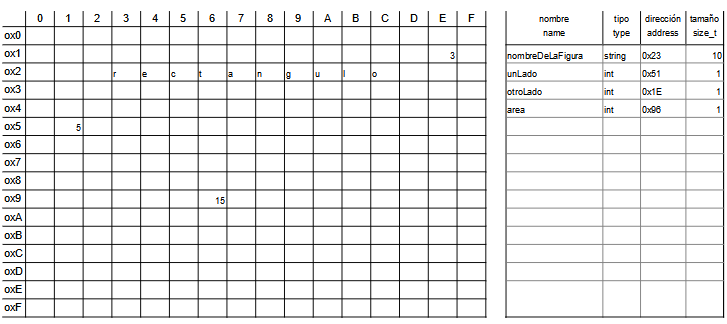
\includegraphics[width=\textwidth]{variables vs celdas de memoria}

\begin{lstlisting}[frame=single, caption=lenguaje Python]

def main(args):
    nombreDeLaFigura = "rectangulo"
    unLado = 5
    otroLado = 3
    area = unLado * otroLado
    
    print(f"Un {nombreDeLaFigura}",
          f"de {unLado} x {otroLado}",
          f"tiene un area de {area}")
    return 0

if __name__ == '__main__':
    import sys
    sys.exit(main(sys.argv))
    
\end{lstlisting}

\begin{lstlisting}[frame=single, caption=lenguaje Java]

public class Variables {
	
    public static void main (String[] args) {
        String nombreDeLaFigura = "rectangulo";
        Integer unLado;
        unLado = 5;
        Integer otroLado;
        otroLado = 3;
        Integer area;
        area = unLado * otroLado;
        
        System.out.println("Un " + nombreDeLaFigura
                           + " de " + unLado
                           + " x " + otroLado 
                           + " tiene un area de " + area);

    }
	
}

\end{lstlisting}

\begin{lstlisting}[frame=single, caption=lenguaje C\#]

using System;

namespace pruebas
{

    class Variables
    {
    
        static void Main(string[] args)
        {
            string nombreDeLaFigura = "rectangulo" 
            int unLado
            unLado = 5;
            int otroLado
            otroLado = 3;
            int area;
            area = unLado * otroLado;
            
            Console.WriteLine("Un " + nombreDeLaFigura 
                              + " de " + unLado
                              + " x " + otroLado 
                              + " tiene un area de " + area);
        }
        
    }
    
}


    
\end{lstlisting}

\begin{lstlisting}[frame=single, caption=lenguaje C]

#include <stdio.h>

int main(int argc, char **argv)
{
    char nombreDeLaFigura[] = "rectanculo";
    int unLado;
    unLado = 5;
    int otroLado;
    otroLado = 3;
    int area;
    area = unLado * otroLado;
    
    printf("Un %s de %i x %i tiene un area de %i",
           nombreDeLaFigura, unLado, otroLado, area);
    return 0;
}
\end{lstlisting}

\begin{lstlisting}[frame=single, caption=lenguaje C++]

#include <iostream>
#include <string>

int main(int argc, char **argv)
{
    std::string nombreDeLaFigura = "rectanculo";
    int unLado = 5;
    int otroLado = 3;
    int area;
    area = unLado * otroLado;
    
    std::cout <<  "Un " << nombreDeLaFigura 
              << " de " << unLado << " x " << otroLado 
              << " tiene un area de " << area;
    return 0;
}



\end{lstlisting}

 
El tratamiento de los tipos de datos depende mucho del lenguaje:
\begin{itemize}
\item Algunos exigen que se indique expresamente el tipo de todas y cada una de las variables.
\item Otros deducen el tipo a partir del primer dato que se asigne a la variable. 
\item Otros utilizan variables de tipo ``generico'' válidas para cualquier tipo.
\item Algunos realizan de forma automática las conversiones de tipo necesarias en las operaciones. 
\item Otros solo permiten conversiones explícitas y dan error cuando los tipos ``no casan'' en alguna operación.
\end{itemize}

Por ejemplo. En los diferentes códigos mostrados antes se han multiplicado dos números enteros (los lados) y se ha asignado el resultado a otro número entero (el área). Pero, ¿qué pasará si se intenta calcular la división de dos números enteros?. O, en el propio caso de la multiplicación, ¿si uno de los lados es entero pero el otro tiene decimales?\ldots



\section{El concepto de `alcance' (scope)}
Alcance (scope) $\rightarrow$ saber en qué parte del código ``vive'' (es válida) una determinada variable o una determinada función.

Como regla general, una variable o una  función solo es válida dentro del ``bloque'' en que ha sido definida (declarada).

\vspace{1cm}
Por eso, es una buena costumbre declarar las variables allá donde se vayan a utilizar por primera vez. De esta forma, ayudamos a limitar su vida solo al bloque donde sean necesarias. 
\\Y, de paso, destacan claramente aquellas variables que o bien tienen un alcance demasiado pequeño --no podemos utilizarla en algún sitio donde la necesitamos--, o bien tienen un alcance demasiado grande --la estamos utilizando en sitios demasiado alejados de donde ha sido declarada--.

nota: Por bloque, se entienden estructuras tales como: cada rama de una condicional, cada rama de una selección, cada bucle, cada función,\ldots
\\nota: Este concepto de alcance permite tener dos variables con exactamente el mismo nombre, siempre que sus alcances no se solapen (estén en bloques distintos). Pero, en general, casi siempre es mejor usar nombres distintos (y descriptivos).


\section{Una variable puede contener un valor simple o un valor compuesto}
Todos los lenguajes traen predefinidos unos tipos básicos de datos nativos: números enteros, números decimales, textos, fechas, etc.

\begin{itemize}
\item Python: \url{https://docs.python.org/3/reference/datamodel.html#the-standard-type-hierarchy}
\item Java: \url{https://docs.oracle.com/javase/specs/jls/se16/html/jls-4.html#jls-4.2}
\item C\#: \url{https://docs.microsoft.com/es-es/dotnet/csharp/language-reference/builtin-types/value-types#built-in-value-types}
\item C: \url{https://en.cppreference.com/w/c/language/type}
\item C++: \url{https://en.cppreference.com/w/cpp/language/type}
\end{itemize}

\vspace{0.5cm}
Y, además, todos los lenguajes suelen contar con mecanismos para definir nuevos tipos de datos personalizados ``ad-hoc''. Esos tipos de datos personalizados pueden contemplar datos compuestos, con múltiples campos en su interior.

Por ejemplo, una dirección\_postal con: calle, portal, piso, codigo\_postal, poblacion, provincia y pais.

O, por ejemplo, un registro de un sensor con: identificación del sensor, momento de la lectura, valor de temperatura y valor de humedad.

  

\begin{lstlisting}[frame=single, caption=lenguaje Python]
from collections import namedtuple


def main(args):
    DireccionPostal = namedtuple(
        "DireccionPostal",
        "calle, portal, piso, codigo_postal, poblacion, provincia, pais")

    mi_casa = DireccionPostal("c/ Pruebas", "2B", "5to izda",
                              "20999", "PuebloPruebas", "ProvinciaPruebas", "PaisPruebas")

    tu_casa = DireccionPostal("c/ Experimentos", "3", "2do dcha",
                              "20789", "PuebloExp", "ProvinciaExp", "PaisExp")

    print(f"Yo vivo en: {mi_casa}")
    print(f"Y tu vives en: {tu_casa}")
    print(f"Mi piso es {mi_casa.piso} y el tuyo es {tu_casa.piso}")

    return 0


if __name__ == '__main__':
    import sys
    sys.exit(main(sys.argv))
\end{lstlisting}

\begin{lstlisting}[frame=single]
Yo vivo en: DireccionPostal(calle='c/ Pruebas', portal='2B', piso='5to izda', codigo_postal='20999', poblacion='PuebloPruebas', provincia='ProvinciaPruebas', pais='PaisPruebas')
Y tu vives en: DireccionPostal(calle='c/ Experimentos', portal='3', piso='2do dcha', codigo_postal='20789', poblacion='PuebloExp', provincia='ProvinciaExp', pais='PaisExp')
Mi piso es 5to izda y el tuyo es 2do dcha
\end{lstlisting}

\begin{lstlisting}[frame=single, caption=lenguaje C]

#include <stdio.h>

int main(int argc, char **argv)
{
    struct DireccionPostal 
    {
        char *calle;
        char *portal;
        char *piso;
        char *codigo_postal;
        char *poblacion;
        char *provincia;
        char *pais;
    };
    
    struct DireccionPostal mi_casa = { .calle="c/ Pruebas",
                                       .portal="2B",
                                       .piso="5to izda",
                                       .codigo_postal="20999",
                                       .poblacion="PuebloPruebas",
                                       .provincia="ProvinciaPruebas",
                                       .pais="PaisPruebas" };
                              
    struct DireccionPostal tu_casa = { .calle="c/ Experimentos",
                                       .portal="3",
                                       .piso="2do dcha",
                                       .codigo_postal="20789",
                                       .poblacion="PuebloExp",
                                       .provincia="ProvinciaExp",
                                       .pais="PaisExp" };
                              
    printf("Yo vivo en: \n %s %s; %s \n %s - %s \n %s(%s) \n",
           mi_casa.calle, mi_casa.portal, mi_casa.piso,
           mi_casa.codigo_postal, mi_casa.poblacion,
           mi_casa.provincia, mi_casa.pais);
    printf("\n"); 
    printf("Y tu vives en: \n %s %s; %s \n %s - %s \n %s(%s) \n",
           tu_casa.calle, tu_casa.portal, tu_casa.piso,
           tu_casa.codigo_postal, tu_casa.poblacion,
           tu_casa.provincia, tu_casa.pais);
    printf("\n"); 
    printf("Mi piso es %s y el tuyo es %s \n", mi_casa.piso, tu_casa.piso);  
    
	
    return 0;
}
\end{lstlisting}
\begin{lstlisting}[frame=single]
Yo vivo en:
 c/ Pruebas 2B; 5to izda
 20999 - PuebloPruebas
 ProvinciaPruebas(PaisPruebas)

Y tu vives en:
 c/ Experimentos 3; 2do dcha
 20789 - PuebloExp
 ProvinciaExp(PaisExp)

Mi piso es 5to izda y el tuyo es 2do dcha
\end{lstlisting}


\begin{lstlisting}[frame=single, caption=lenguaje Python]
from collections import namedtuple
from datetime import datetime


def main(args):
    LecturaSensorTH = namedtuple("LecturaSensorTH",
                                 "sensor_ID, timestamp, temperatura_gradosC, humedad_relativa")

    una_lectura = LecturaSensorTH("SALON",
                                  datetime(year=2021, month=7, day=16,
                                           hour=13, minute=33, second=45),
                                  21.3, 58)

    otra_lectura = LecturaSensorTH("COCINA",
                                   datetime(year=2020, month=11, day=1,
                                            hour=22, minute=48, second=15),
                                   2.9, 27)

    print(f"Tenemos guardado en el sistema:")
    print(f"   {una_lectura}")
    print(f"   {otra_lectura}")
    print()
    fecha = una_lectura.timestamp.strftime("%Y/%m/%d")
    hora = una_lectura.timestamp.strftime("%H:%M:%S")
    print(f"El dia {fecha} a las {hora} habia",
          f"una temperatura de {una_lectura.temperatura_gradosC} grados Celsius",
          f"y {una_lectura.humedad_relativa} % de humedad en: {una_lectura.sensor_ID}")

    return 0


if __name__ == '__main__':
    import sys
    sys.exit(main(sys.argv))
\end{lstlisting}

\begin{lstlisting}[frame=single]
Tenemos guardado en el sistema:
   LecturaSensorTH(sensor_ID='SALON', timestamp=datetime.datetime(2021, 7, 16, 13, 33, 45), temperatura_gradosC=21.3, humedad_relativa=58)
   LecturaSensorTH(sensor_ID='COCINA', timestamp=datetime.datetime(2020, 11, 1, 22, 48, 15), temperatura_gradosC=2.9, humedad_relativa=27)

El dia 2021/07/16 a las 13:33:45 habia una temperatura de 21.3 grados Celsius y 58 % de humedad en: SALON
\end{lstlisting}

\begin{lstlisting}[frame=single, caption=lenguaje C]
#include <stdio.h>
#include <time.h>

int main(int argc, char **argv)
{
    struct LecturaSensorTH
    {
        char *sensor_ID;
        struct tm *timestamp;
        double temperatura_gradosC;
        int humedad_relativa;
    };

    struct tm un_momento = 
                      { .tm_year = 2021, .tm_mon = 7, .tm_mday = 16,
                        .tm_hour = 13, .tm_min = 33, .tm_sec = 45};
                        
    struct LecturaSensorTH una_lectura =
                                    { .sensor_ID = "SALON",
                                      .timestamp = &un_momento,
                                      .temperatura_gradosC = 21.3,
                                      .humedad_relativa = 58};

    struct tm otro_momento = 
                      { .tm_year = 2020, .tm_mon = 11, .tm_mday = 1,
                        .tm_hour = 22, .tm_min = 48, .tm_sec = 15};

    struct LecturaSensorTH otra_lectura =
                                    { .sensor_ID = "COCINA",
                                      .timestamp = &otro_momento,
                                      .temperatura_gradosC = 2.9,
                                      .humedad_relativa = 27};

    printf("Tenemos guardado en el sistema: \n");
    printf("   %s %s %f %d \n", una_lectura.sensor_ID,
                                asctime(una_lectura.timestamp),
                                una_lectura.temperatura_gradosC,
                                una_lectura.humedad_relativa);
    printf("   %s %s %f %d \n", otra_lectura.sensor_ID,
                                asctime(otra_lectura.timestamp),
                                otra_lectura.temperatura_gradosC,
                                otra_lectura.humedad_relativa);
    printf("\n");
    printf("El dia %d/%d/%d a las %d:%d:%d habia %f grados Celsius y %d %% de humedad en la %s",
           una_lectura.timestamp->tm_year,
           una_lectura.timestamp->tm_mon,
           una_lectura.timestamp->tm_mday,
           una_lectura.timestamp->tm_hour,
           una_lectura.timestamp->tm_min,
           una_lectura.timestamp->tm_sec,
           una_lectura.temperatura_gradosC,
           una_lectura.humedad_relativa,
           una_lectura.sensor_ID);
    
    return 0;
}
\end{lstlisting}

\begin{lstlisting}[frame=single]
Tenemos guardado en el sistema:
   SALON Sun Aug 16 13:33:45 3921
 21.300000 58
   COCINA Sun Dec 01 22:48:15 3920
 2.900000 27

El dia 2021/7/16 a las 13:33:45 habia 21.300000 grados Celsius y 58 % de humedad en la SALON
\end{lstlisting}


\section{Algunos consejos prácticos}

\subsection{La importancia de poner nombres claros y descriptivos a las variables.}
Cualquier persona pasa más tiempo leyendo código que escribiéndolo.

La claridad y facilidad de lectura del propio código ayuda mucho a la mantenibilidad del programa. 

Evitar poner nombres demasiado cortos (abreviaturas difíciles de entender) o nombres demasiado genéricos (difíciles de relacionar con su significado real).

Si un programa necesita de comentarios \footnote{La misión de los comentarios en el código no es indicar lo que este hace. Los comentarios son para aclarar aquellos asuntos difíciles de deducir leyendo el propio código. Por ejemplo: indicar por qué se ha optado por una extraña construcción muy inusual; avisar del extraño comportamiento de algún dispositivo externo que se está utilizando; etc.} para explicarlo, algo anda mal en ese código\ldots




\subsection{La importancia de los tipos de datos.}
Los ordenadores tienen ciertas limitaciones al almacenar información: precisión numérica, codificación de caracteres,\ldots. De ahí que cada variable tenga asociado un tipo de dato concreto (una forma concreta de almacenar su valor en memoria).

Al convertir un tipo en otro (por ejemplo, al almacenar el valor de una variable de un tipo en otra variable de otro tipo) pueden surgir problemas: resultados incorrectos en cálculos por pérdida de precisión al truncar cifras significativas, aparición de caracteres extraños en los textos,\ldots

Algunos lenguajes son muy estrictos con los tipos, obligando a realizar de forma explícita todas las conversiones (``cast''). Mientras que otros dan mucha más libertad y realizan (o intentan realizar) de forma automática las conversiones necesarias.

Pero, en el fondo, todos los lenguajes han de lidiar con las limitaciones de las representaciones binarias de datos en memoria. Y, por eso es importante conocer al menos algo sobre cómo maneja estos temas el lenguaje en el que estemos programando.





\chapter{La consola de comandos: el interfaz de usuario más simple.}


\section{Mostrar texto en la pantalla}
Mostrar información (textos, números,\ldots) en pantalla suele ser sencillo. Pero  la cosa se complica cuando deseamos manejar los diversos ``usos y costumbres'' alrededor del mundo. Por ejemplo:
\begin{itemize}
\item En los números, ¿separador decimal con coma o con punto?, ¿delimitadores de miles con puntos o con comas?.
\item En números resultado de operaciones con otros números (por ejemplo totales), ¿redondear los propios números antes de operar con ellos? ¿redondear solo lo presentado en pantalla? (si la persona usa una calculadora para calcular lo que ve en pantalla, muy posiblemente los resultados no le cuadren).
\item En las fechas, ¿va primero el día, luego el mes y luego el año?, ¿o va primero el mes, luego el día y luego el año?, ¿o\ldots?
\end{itemize}

Por ejemplo, para mostrar esto en pantalla:
\begin{lstlisting}
Mostrar el numero tal cual:  2.7285
Mostrarlo con solo dos decimales: 2.73

Fecha segun formato automático del pais de donde seas:  domingo, 28/05/1967
Fecha segun formato aleman:  Sonntag, 28.05.1967
Fecha segun fomato estadounidense:  Sunday, 5/28/1967
Fecha segun un cierto formato determinado:  1967/05/28
\end{lstlisting}

Podemos usar alguno de estos programas:

\begin{lstlisting}[frame=single, caption=lenguaje python]

import locale
import datetime


def main(args):

    unNumero = 2.7285
    print(f"Mostrar el numero tal cual: {unNumero}")
    print(f"Mostrarlo con solo dos decimales: {unNumero:.2f}")

    print()

    miFechaDeNacimiento = datetime.date(1967, 5, 28)

    locale.setlocale(locale.LC_TIME, "")
    print("Fecha segun formato automático del pais de donde seas: ",
          f"{miFechaDeNacimiento.strftime('%A, %x')}")

    locale.setlocale(locale.LC_TIME, "de_DE")
    print("Fecha segun formato aleman: ",
          f"{miFechaDeNacimiento.strftime('%A, %x')}")

    locale.setlocale(locale.LC_TIME, "us_US")
    print("Fecha segun fomato estadounidense: ",
          f"{miFechaDeNacimiento.strftime('%A, %x')}")
    locale.setlocale(locale.LC_TIME, "")

    print("Fecha segun un cierto formato determinado: ",
          f"{miFechaDeNacimiento.strftime('%Y/%m/%d')}")

    return 0


if __name__ == '__main__':
    import sys
    sys.exit(main(sys.argv))
\end{lstlisting}


\begin{lstlisting}[frame=single, caption=lenguaje java]

import java.time.LocalDate;
import java.time.format.DateTimeFormatter;
import java.time.format.FormatStyle;


public class textoPorConsola {
	
    public static void main (String[] args) {
        
        Double unNumero = 2.7828;
        System.out.println("Mostrar el numero tal cual: " + unNumero);
        System.out.format("Mostrarlo con solo dos decimales: %.2f %n", unNumero);
        
        System.out.println();
       
        LocalDate miFechaDeNacimiento = LocalDate.of(1967, 5, 28);

        DateTimeFormatter formateadorBase = DateTimeFormatter.ofLocalizedDate(FormatStyle.FULL);
        System.out.println("Fecha segun formato automático del pais de donde seas: "
                           + formateadorBase.format(miFechaDeNacimiento));

        DateTimeFormatter formateadorAleman = formateadorBase.localizedBy(java.util.Locale.GERMANY);
        System.out.println("Fecha segun formato aleman: "
                           + formateadorAleman.format(miFechaDeNacimiento));
             
        DateTimeFormatter formateadorEEUU = formateadorBase.localizedBy(java.util.Locale.US);
        System.out.println("Fecha segun formato estadounidense: "
                           + formateadorEEUU.format(miFechaDeNacimiento));

        DateTimeFormatter formateadorManual = DateTimeFormatter.ofPattern("YYYY/MM/dd");
        System.out.println("Fecha segun un cierto formato determinado: "
                           + formateadorManual.format(miFechaDeNacimiento));
        System.out.format("Tambien se puede hacer asi: %1$tY/%1$tm/%1$te %n", miFechaDeNacimiento); 


    }
    
}
\end{lstlisting}

\begin{lstlisting}[frame=single, caption=lenguaje C\#]
using System;
using System.Globalization;

namespace ConsoleApp1
{
    class TextoPorConsola
    {
        static void Main(string[] args)
        {

            Double unNumero = 2.7828;
            Console.WriteLine("Mostrar el numero tal cual: " + unNumero);
            Console.WriteLine("Mostrarlo con solo dos decimales: " + unNumero.ToString("F2"));

            Console.WriteLine();

            DateTime miFechaDeNacimiento = new DateTime(1967, 5, 28);

            Console.WriteLine("Fecha segun formato automático del pais de donde seas: "
                              + miFechaDeNacimiento.ToLongDateString());

            CultureInfo culturaAlemana = CultureInfo.CreateSpecificCulture("de-DE");
            Console.WriteLine("Fecha segun formato aleman: "
                              + miFechaDeNacimiento.ToString("D", culturaAlemana));

            CultureInfo culturaEEUU = CultureInfo.CreateSpecificCulture("en-US");
            Console.WriteLine("Fecha segun formato estadounidense: "
                              + miFechaDeNacimiento.ToString("D", culturaEEUU));

            Console.WriteLine("Fecha segun un cierto formato determinado: "
                              + miFechaDeNacimiento.ToString("yyyy/MM/dd"));

        }

    }
}

\end{lstlisting}


A título meramente ilustrativo, sin pretender asustar, solo para mostrar la complejidad del tema.  Algunos ejemplos de documentación sobre cómo formatear números, cantidades y fechas/tiempo:

En Python
\\ \url{https://docs.python.org/3/library/string.html#formatspec}
\\ \url{https://docs.python.org/3/library/datetime.html#strftime-strptime-behavior}

En java
\begin{footnotesize}
\\ \url{https://docs.oracle.com/en/java/javase/16/docs/api/java.base/java/time/format/DateTimeFormatter.html}
\end{footnotesize}

En C\#
\begin{scriptsize}
\\ \url{https://docs.microsoft.com/es-es/dotnet/standard/base-types/standard-numeric-format-strings}
\\ \url{https://docs.microsoft.com/es-es/dotnet/api/system.globalization.datetimeformatinfo?view=net-5.0#format-strings-and-datetimeformatinfo-properties}
\end{scriptsize}

En C++
\begin{footnotesize}
\\ \url{https://www.cplusplus.com/reference/locale/}
\\ \url{https://en.cppreference.com/w/cpp/locale}
\end{footnotesize}

\section{Recoger lo que se teclea en el teclado}
Recoger texto tecleado por el usuario es sencillo. La complicación llega a la hora de:
\begin{itemize}
\item Interpretar la información contenida en el texto: números con decimales, números con separadores de miles, números con unidades, cantidades monetarias con indicación de moneda, fechas en diversos formatos, etc.
\item Interpretar las teclas de navegación para implementar un diálogo no lineal, que permita al usuario posicionarse en un punto concreto de la pantalla para introducir información en campos concretos de un formulario.
\end{itemize}
 
Por ejemplo, para elaborar un diálogo lineal simple como este:
\begin{lstlisting}
Introduce tu nombre: Juan
Introduce un numero entero: 236
Introduce un numero con decimales: 12.9842

Muchas gracias,  Juan , por haber introducido los numeros  236  y  12.9842
\end{lstlisting}

Podemos usar alguno de estos programas:

\begin{lstlisting}[frame=single, caption=lenguaje phyton]

def main(args):
    
    nombreDelUsuario = input("Introduce tu nombre: ")
    unNumeroEntero = int(input("Introduce un numero entero: "))
    unNumeroDecimal = float(input("Introduce un numero con decimales: "))
    
    print()
    print("Muchas gracias, ", nombreDelUsuario, 
          ", por haber introducido los numeros ",
          unNumeroEntero, " y ", unNumeroDecimal)
    
    return 0

if __name__ == '__main__':
    import sys
    sys.exit(main(sys.argv))
\end{lstlisting}



\begin{lstlisting}[frame=single, caption=lenguaje java]

public class entradaPorConsola {
	
    public static void main (String[] args) {
		
        java.util.Scanner lectorDeTeclado = new java.util.Scanner(System.in);
        
        System.out.println("Introduce tu nombre: ");
        String nombreDelUsuario = lectorDeTeclado.nextLine();
        
        System.out.println("Introduce un numero entero: ");
        Integer unNumeroEntero = lectorDeTeclado.nextInt();
        
        System.out.println("Introduce un numero con decimales: ");
        Double unNumeroDecimal = lectorDeTeclado.nextDouble();
        
        System.out.println();
        System.out.println("Muchas gracias, " + nombreDelUsuario 
                           + ", por haber introducido los numeros "
                           + unNumeroEntero + " y " + unNumeroDecimal);
	
    }
    
}
\end{lstlisting}

\begin{lstlisting}[frame=single, caption=lenguaje C\#]
using System;

namespace ConsoleApp1
{
    class EntradaPorConsola
    {
        static void Main(string[] args)
        {
            Console.WriteLine("Introduce tu nombre: ");
            String nombreDelUsuario = Console.ReadLine();

            Console.WriteLine("Introduce un numero entero: ");
            Int32 unNumeroEntero = Int32.Parse(Console.ReadLine());

            Console.WriteLine("Introduce un numero con decimales: ");
            Double unNumeroDecimal = Double.Parse(Console.ReadLine());

            Console.WriteLine();
            Console.WriteLine("Muchas gracias, " + nombreDelUsuario
                               + ", por haber introducido los numeros "
                               + unNumeroEntero + " y " + unNumeroDecimal);

        }

    }
}
\end{lstlisting}


\begin{lstlisting}[frame=single, caption=lenguaje C++]
#include <iostream>
#include <string>

int main(int argc, char **argv)
{
    std::string nombreDelUsuario;
    std::cout << "Introduce tu nombre: ";
    std::cin >> nombreDelUsuario;

    int unNumeroEntero;
    std::cout << "Introduce un numero entero: ";
    std::cin >> unNumeroEntero;

    float unNumeroDecimal;
    std::cout << "Introduce un numero con decimales: ";
    std::cin >> unNumeroDecimal;

    std::cout << std::endl
              << "Muchas gracias, " << nombreDelUsuario
              << ", por haber introducido los numeros " 
              << unNumeroEntero << " y " << unNumeroDecimal
              << std::endl;

    return 0;
}
\end{lstlisting}



\begin{lstlisting}[frame=single, caption=lenguaje C]
#include <stdio.h>

int main(int argc, char **argv)
{
    int LONGITUD_MAXIMA_DEL_NOMBRE = 20;
    char nombreDelUsuario[LONGITUD_MAXIMA_DEL_NOMBRE];
    printf("Introduce tu nombre: ");
    fgets(nombreDelUsuario, LONGITUD_MAXIMA_DEL_NOMBRE, stdin);

    int unNumeroEntero;
    printf("Introduce un numero entero: ");
    scanf("%i", &unNumeroEntero);

    float unNumeroDecimal;
    printf("Introduce un numero con decimales: ");
    scanf("%f", &unNumeroDecimal);

    printf("\n");
    printf("Muchas gracias, %s, por haber introducido los numeros %i y %f",
           nombreDelUsuario, unNumeroEntero, unNumeroDecimal);
	
    return 0;
}

\end{lstlisting}


nota: Hubo un tiempo en que se utilizaban bibliotecas de funciones especializadas para elaborar diálogos textuales más complejos. Por ejemplo \url{https://es.wikipedia.org/wiki/Ncurses}
\\Pero hoy en día lo habitual es utilizar un interfaz gráfico de usuario (GUI, Graphic User Interface) en lugar de estos interfaces textuales. Pero eso\ldots es otra historia\ldots


\chapter{El flujo de ejecución: cómo gobernar lo que se va ejecutando.}

\section{Ramas condicionales: IF/ELSE}
Se utilizan para ejecutar o no cierto grupo de instrucciones según se cumpla o no una cierta condición.

``IF'' $\rightarrow$ SI
\\``ELSE'' $\rightarrow$ SI NO

\begin{lstlisting}
IF (condicion)
    cosas a hacer si se cumple la condición
ELSE
    cosas a hacer si no se cumple
\end{lstlisting}
nota: La parte ELSE es opcional.

nota: En Pyton, la instrucción `elif' equivale a `ELSE IF'; y se utiliza para encadenar comprobaciones una detrás de otra.
\begin{lstlisting}[frame=single, caption=lenguaje python]
import math


def main(args):

    opcion = int(
        input("¿(1) rectangulo o (2) circunferencia? Elija una opción: "))

    if (opcion == 1):
        unlado = float(input("Introduzca la medida de un lado: "))
        otrolado = float(input("Introduzca la medida del otro lado: "))
        area = unlado * otrolado
        perimetro = unlado * 2 + otrolado * 2
        print(f"Ese rectangulo tiene un area de {area:.4f}",
              f" y un perimetro de {perimetro:.4f}")
    elif (opcion == 2):
        radio = float(input("Introduzca el radio: "))
        area = math.pi * radio ** 2
        perimetro = 2 * math.pi * radio
        print(f"Esa circunferencia tiene un area de {area:.4f}",
              f" y un perimetro de {perimetro:.4f}")
    else:
        print(f"Solo se admite 1 o 2 como opción. ",
              f"{opcion} no esta contemplado.")

    return 0


if __name__ == '__main__':
    import sys
    sys.exit(main(sys.argv))
\end{lstlisting}
\begin{lstlisting}[frame=single]
?(1) rectangulo o (2) circunferencia? Elija una opción: 2
Introduzca el radio: 12
Esa circunferencia tiene un area de 452.3893  y un perimetro de 75.3982

?(1) rectangulo o (2) circunferencia? Elija una opción: 1
Introduzca la medida de un lado: 2
Introduzca la medida del otro lado: 3
Ese rectangulo tiene un area de 6.0000  y un perimetro de 10.0000

?(1) rectangulo o (2) circunferencia? Elija una opción: 4
Solo se admite 1 o 2 como opción.  4 no esta contemplado.
\end{lstlisting}

\begin{lstlisting}[frame=single, caption=lenguaje java]

public class IfyElse {
	
    public static void main (String[] args) {
        java.util.Scanner lectorDeTeclado = new java.util.Scanner(System.in);
        
        System.out.println("(1) rectangulo o (2) circunferencia? Elija una opcion: ");
        Integer opcion = lectorDeTeclado.nextInt();

        if(opcion == 1) {
            System.out.println("Introduzca la medida de un lado: ");
            Double unlado = lectorDeTeclado.nextDouble();
            System.out.println("Introduzca la medida del otro lado: ");
            Double otrolado = lectorDeTeclado.nextDouble();   

            Double area = unlado * otrolado;
            Double perimetro = unlado * 2 + otrolado * 2;
            System.out.format("Ese rectangulo tiene un area de %.4f"
                              + " y un perimetro de %.4f", area, perimetro);
        }
        else if(opcion == 2) {
            System.out.println("Introduzca el radio: ");
            Double radio = lectorDeTeclado.nextDouble();

            Double area = Math.PI * radio * radio;
            Double perimetro =  2 * Math.PI * radio;
            System.out.format("Esa circunferencia tiene un area de %.4f"
                              + " y un perimetro de %.4f", area, perimetro);
        }
        else {
            System.out.println("Solo se admite 1 o 2 como opción. " 
                               + opcion + " no esta contemplado.");
        }
        
    }
    
}

\end{lstlisting}


\begin{lstlisting}[frame=single, caption=lenguaje C\#]
using System;

namespace ConsoleApp1
{
    class IfyElse
    {
        static void Main(string[] args)
        {
            Console.WriteLine("(1) rectangulo o (2) circunferencia? Elija una opcion: ");
            Byte opcion = Byte.Parse(Console.ReadLine());

            if (opcion == 1)
            {
                Console.WriteLine("Introduzca la medida de un lado: ");
                Double unlado = Double.Parse(Console.ReadLine());
                Console.WriteLine("Introduzca la medida del otro lado: ");
                Double otrolado = Double.Parse(Console.ReadLine());

                Double area = unlado * otrolado;
                Double perimetro = unlado * 2 + otrolado * 2;
                Console.WriteLine("Ese rectangulo tiene un area de " + area.ToString("F4")
                                  + " y un perimetro de " + perimetro.ToString("F4"));
            }
            else if (opcion == 2)
            {
                Console.WriteLine("Introduzca el radio: ");
                Double radio = Double.Parse(Console.ReadLine());

                Double area = Math.PI * radio * radio;
                Double perimetro = 2 * Math.PI * radio;
                Console.WriteLine("Esa circunferencia tiene un area de  " + area.ToString("F4")
                                  + " y un perimetro de " + perimetro.ToString("F4"));
            }
            else
            {
                Console.WriteLine("Solo se admite 1 o 2 como opción. "
                                  + opcion + " no esta contemplado.");
            }
        }
    }
}
\end{lstlisting}


\section{Múltiples ramas condicionales: SWITCH}
La instrucción switch se suele utilizar para evitar grandes concatenaciones de construcciones IF/ELSE

nota: El lenguaje Python no implementa una instrucción `switch', se suelen utilizar concatenaciones de `if \ldots elif \ldots elif \ldots elif \ldots else' todo lo largas que sean necesarias.
\begin{lstlisting}[frame=single, caption=lenguaje python]

def main(args):
    palabra = input("Teclee una palabra: ")
    palabraTodoMayusculas = palabra.upper()
    letraInicial = palabraTodoMayusculas[0]
    
    if(letraInicial == 'A'):
        respuesta = "abracadabra"
    elif(letraInicial == 'B'):
        respuesta = "branquia"
    elif(letraInicial == 'C'):
        respuesta = "cabraloca"
    elif(letraInicial == 'D'):
        respuesta = "dodecaedro"
    elif(letraInicial == 'E'):
        respuesta = "especialidad"
    elif(letraInicial == 'F'):
        respuesta = "frio"
    #Aquí seguiriamos poniendo elifs con el resto del alfabeto...
    print("¡Que casualidad!, otra que tambien empieza por esa letra es: ", respuesta)

    return 0


if __name__ == '__main__':
    import sys
    sys.exit(main(sys.argv))
\end{lstlisting}


\begin{lstlisting}[frame=single, caption=lenguaje java]

public class Switch {
	
    public static void main (String[] args) {
        java.util.Scanner lectorDeTeclado = new java.util.Scanner(System.in);
        
        System.out.println("Teclee una palabra: ");
        String palabra = lectorDeTeclado.nextLine();
        
        String palabraTodoMayusculas = palabra.toUpperCase();
        char letraInicial = palabraTodoMayusculas.charAt(0);
        
        String respuesta = "";
        switch(letraInicial) {
            case 'A':
                respuesta = "abracadabra";
                break;
            case 'B':
                respuesta = "branquia";
                break;
            case 'C':
                respuesta = "cabraloca";
                break;
            case 'D':
                respuesta = "dodecaedro";
                break;
            case 'E':
                respuesta = "especialidad";
                break;
            case 'F':
                respuesta = "frio";
                break;
            //Aquí seguiriamos poniendo cases con el resto del alfabeto...
        }
        System.out.println("¡Que casualidad!, otra que tambien empieza por esa letra es: "
                           + respuesta);
		
    }
}


\end{lstlisting}




\section{Bucles condicionales: WHILE}
Se utilizan para ejecutar repetidamente un cierto grupo de instrucciones, hasta que se cumpla una cierta condición.

``WHILE'' $\rightarrow$ MIENTRAS
\begin{lstlisting}
WHILE (condicion)
    cosas a hacer mientras se cumpla la condición
\end{lstlisting}
nota: Si la condición no se cumple al entrar al bucle, el bucle while no hace nada.

nota: Algunos lenguajes  tienen también la instrucción ``UNTIL'' $\rightarrow$ HASTA QUE. Es parecida, solo que la condición se comprueba al final del bucle en lugar de al principio. De esta forma las cosas a hacer dentro del bucle se hacen siempre por lo menos una vez.
\begin{lstlisting}
    cosas a hacer mientras se cumpla la condición
UNTIL (condicion)
\end{lstlisting}


\begin{lstlisting}[frame=single, caption=lenguaje python]
import math


def main(args):
    opcion = 0
    while (opcion != 99):
        print()
        print()
        opcion = int(input("?(1) rectangulo o (2) circunferencia"
                           " o (99) terminar? Elija una opción: "))
        if (opcion == 1):
            unlado = float(input("Introduzca la medida de un lado: "))
            otrolado = float(input("Introduzca la medida del otro lado: "))
            area = unlado * otrolado
            perimetro = unlado * 2 + otrolado * 2
            print(f"Ese rectangulo tiene un area de {area:.4f}",
                  f" y un perimetro de {perimetro:.4f}")
        elif (opcion == 2):
            radio = float(input("Introduzca el radio: "))
            area = math.pi * radio ** 2
            perimetro = 2 * math.pi * radio
            print(f"Esa circunferencia tiene un area de {area:.4f}",
                  f" y un perimetro de {perimetro:.4f}")
        elif (opcion != 99):
            print(f"Solo se admite 1 o 2 o 99 como opción. ",
                  f"{opcion} no esta contemplado.")
        return 0


if __name__ == '__main__':
    import sys
    sys.exit(main(sys.argv))
\end{lstlisting}

\begin{lstlisting}[frame=single, caption=lenguaje java]

public class While {
	
    public static void main (String[] args) {
        java.util.Scanner lectorDeTeclado = new java.util.Scanner(System.in);
        
        Integer opcion = 0;
        
        while(opcion != 99) {
            System.out.println();
            System.out.println();
            System.out.println("(1) rectangulo o (2) circunferencia"
                               + " o (99) terminar ?  Elija una opcion: ");
            opcion = lectorDeTeclado.nextInt();

            if(opcion == 1) {
                System.out.println("Introduzca la medida de un lado: ");
                Double unlado = lectorDeTeclado.nextDouble();
                System.out.println("Introduzca la medida del otro lado: ");
                Double otrolado = lectorDeTeclado.nextDouble();   

                Double area = unlado * otrolado;
                Double perimetro = unlado * 2 + otrolado * 2;
                System.out.format("Ese rectangulo tiene un area de %.4f"
                                  + " y un perimetro de %.4f",
                                  area, perimetro);
            }
            else if(opcion == 2) {
                System.out.println("Introduzca el radio: ");
                Double radio = lectorDeTeclado.nextDouble();

                Double area = Math.PI * radio * radio;
                Double perimetro =  2 * Math.PI * radio;
                System.out.format("Esa circunferencia tiene un area de %.4f"
                                  + " y un perimetro de %.4f",
                                  area, perimetro);
            }
            else if(opcion != 99) {
                System.out.println("Solo se admite 1 o 2 o 99 como opcion. " 
                                   + opcion + " no esta contemplado.");
            }
        }
    }
    
}
\end{lstlisting}



\section{Bucles repetitivos: FOR, FOREACH}
Se suelen utilizar para repetir un cierto grupo de instrucciones un número predeterminado de veces, variando el contenido de ciertas variables cada vez.

``FOR'' $\rightarrow$ PARA
\\``FOREACH'' $\rightarrow$ PARA CADA UNO
\begin{lstlisting}
FOR (preparacion del numero de veces)
    cosas a hacer cada vez
\end{lstlisting}

nota: Las máquinas suelen contar partiendo de cero: 0, 1, 2, 3, 4,\ldots De ahí que aparezcan cláusulas de `+ 1' o de `- 1' en muchos bucles y condiciones; para adaptarlos a la forma de contar humana, partiendo de uno: 1, 2, 3, 4, 5,\ldots

\begin{lstlisting}[frame=single, caption=lenguaje python]
def main(args):
    veces_a_repetir = int(input("¿Cuantas veces quieres que lo repita? "))
    for vez in range(veces_a_repetir):
        numero = 5 * (vez + 1)
        print(f"Te lo repito {vez + 1} veces: son {numero}")
    return 0

if __name__ == '__main__':
    import sys
    sys.exit(main(sys.argv))
\end{lstlisting}

El resultado de este programa es:
\\¿Cuantas veces quieres que repita? 4
\\Te lo repito  1  veces: son  5
\\Te lo repito  2  veces: son  10
\\Te lo repito  3  veces: son  15
\\Te lo repito  4  veces: son  20


\begin{lstlisting}[frame=single, caption=lenguaje java]

public class For {
	
    public static void main (String[] args) {
        java.util.Scanner lectorDeTeclado = new java.util.Scanner(System.in);
        
        System.out.println("¿Cuantas veces quieres que lo repita? ");
        Integer vecesARepetir = lectorDeTeclado.nextInt();
        for(int i = 1; i <= vecesARepetir; i++) {
            Integer numero = 5 * i;
            System.out.println("Te lo repito " + i + " veces: son " + numero);
        }
    }
    
}
\end{lstlisting}

--pendiente de poner algunos ejemplos más de código--

 


\chapter{Las estructuras de datos: cómo organizar la información a manejar.}

\section{Colecciones simples de valores: ARRAY}
Se utilizan para almacenar en una variable un cierto grupo de valores de un determinado tipo.

Son útiles si deseamos montar algo simple y sabemos de antemano el tamaño (número de elementos) que va a ocupar cada array.

Al usar un array, recae sobre la persona programadora la responsabilidad de gestionarlo correctamente para asegurarse de que no se utiliza más allá de su tamaño máximo. 

nota: En algunos lenguajes, superar el tamaño máximo del array suele provocar un error. En otros lenguajes, suele provocar la lectura o escritura en posiciones de memoria donde no correspondería hacerlo (el famoso e infame ``buffer overflow'').

¡Importante!: 
\\Hoy en día (año 2021) existen alternativas a los array. Casi todas las bibliotecas estandares, de casi todos los lenguajes, contemplan algún tipo de ``colecciones'' (listas, diccionarios, sets, tuplas,\ldots).
\\ Estas colecciones son como  ``arrays inteligentes'', permitiendo ampliar/reducir automáticamente su tamaño según se va necesitando.
\\ Salvo que se esté programando en un entorno de memoria muy reducida (por ejemplo un sistema embebido con unos pocos Kb. de memoria), donde se necesite gestionar manualmente el almacenamiento en memoria. Es mucho más práctico (y seguro) utilizar alguna de esas colecciones en lugar de arrays.

De todas formas, los array (junto con las listas encadenadas) son la base de la gestión de datos en memoria. Así que es ilustrativo conocer su funcionamiento.


\begin{lstlisting}[frame=single, caption=lenguaje C]

#include <stdio.h>
#include <stdlib.h>
#include <time.h>


int const MAX_LECTURAS = 100;

int getMedidasDelSensorFicticio(float lecturas[], int tamainoDelArrayLecturas);
float getSiguienteMedida();


int main(int argc, char** argv)
{
    srand(time(NULL));

    float lecturas[MAX_LECTURAS];
    int numeroDeLecturas;
    numeroDeLecturas = getMedidasDelSensorFicticio(lecturas, MAX_LECTURAS);

    float suma = 0;
    for (int i = 0; i < numeroDeLecturas; i++)
    {
        suma = suma + lecturas[i];
    }

    float media;
    if (numeroDeLecturas > 0)
    {
        media = suma / numeroDeLecturas;
    }
    else
    {
        media = 0;
    }

    printf("Se han tomado %d medidas en el sensor; su valor medio es %.2f", numeroDeLecturas, media);

    return 0;
}


int getMedidasDelSensorFicticio(float lecturas[], int const tamainoDelArrayLecturas)
{
    int i = 0;
    float lectura;
    do
    {
        lectura = getSiguienteMedida();
        if (lectura >= 0.0)
        {
            lecturas[i] = lectura;
            i++;
        }
    } while ((i < tamainoDelArrayLecturas) && (lectura >= 0.0));
    return i;
}

float getSiguienteMedida()
{
    //Aqui es donde se leeria la cola de medidas en el sensor...
    //Suponemos que el sensor devuelve -1 si no tiene mas medidas almacenadas...
    //Pero para simplificar el ejemplo, en este caso siempre devolvemos un valor aleatorio...
    return rand() / 888.8;
}

\end{lstlisting}


\vspace{1cm}
--pendiente de poner más  ejemplos de código--


\section{Valores predefinidos: ENUM}
Se utilizan para asegurar que una variable contiene solo ciertos valores predefinidos.

Son útiles cuando sabemos de antemano los valores permitidos y deseamos que no se utilicen más que esos valores.


\vspace{1cm}
--pendiente de poner algunos ejemplos de código--


\section{Colecciones de valores:}

\subsection{Listas de valores individuales: LIST}
Son como un array, pero admiten ir ampliando o reduciendo su capacidad sobre la marcha. En cierto modo son como una especie de array ``ilimitado''.

En su interior suelen funcionar con alguna variante de `lista encadenada' (\url{https://es.wikipedia.org/wiki/Lista_enlazada}). Pero en su uso práctico tan solo nos hemos de preocupar en añadir (add) o quitar (remove) elementos.

Dependiendo del lenguaje de programación y de la biblioteca de funciones utilizada, las listas pueden incorporar funciones de utilidad tales como: insertar un elemento entre dos existentes, ordenar todos los elementos, buscar un elemento concreto, etc.

Pero se ha de tener en cuenta que las listas están optimizadas para ser recorridas de forma secuencial, elemento a elemento; y no para acceder a elementos concretos de forma individual (para eso están los diccionarios).

\begin{lstlisting}[frame=single, caption=lenguaje java]

public class TrabajoConListas {
	
    public static void main (String[] args) {
        SensorFicticio sensor = new SensorFicticio();
        java.util.ArrayList<Double> lecturas = sensor.getMedidas();
        
        Double suma = 0;
        for (Double valor :lecturas) {
            suma = suma + valor;
        }
        
        Double media;
        if (lecturas.size() > 0) {
            media = suma / lecturas.size();
        }
        else {
            media = 0;
        }
        
        System.out.format("Se han tomado %d medidas en el sensor; su valor medio es %.2f", lecturas.size(), media);
    }
    
}


public class SensorFicticio {
    
    public java.util.ArrayList<Double> getMedidas() {
        java.util.ArrayList<Double> lecturas = new java.util.ArrayList<Double>();
        Double lectura;
        do {
            lectura = getSiguienteMedida();
            if (lectura >= 0.0) {
                lecturas.add(lectura);
            }
        } while (lectura >= 0.0);
        return lecturas;
    }
    
    
    private Double getSiguienteMedida() {
        //Aqui es donde se leeria en el sensor...
        //Suponemos que el sensor devuelve -1.0 si no tiene mas medidas almacenadas...
        //Para simplificar, lo simularemos con numeros aleatorios...
        Double valor = Math.random() * 200;
        if (valor > 50 && valor < 55) {
            return -1.0;
        }
        else {
            return valor;
        }
    }
    
}


\end{lstlisting}

\begin{lstlisting}[frame=single, caption=lenguaje C++]

#include <iostream>
#include <vector>
#include <chrono>
#include <random>


class SensorFicticio
{
    
public:

std::vector<float> getMedidas()
{
    std::vector<float> lecturas;
    float lectura;
    do
    {
        lectura = getSiguienteMedida();
        if (lectura >= 0.0)
        {
            lecturas.push_back(lectura);
        }
    } while (lectura >= 0.0);
    return lecturas;
}


private:

float getSiguienteMedida()
{
    //Aqui es donde se leeria en el sensor...
    //Suponemos que el sensor devuelve -1.0 si no tiene mas medidas almacenadas...
    //Para simplificar, lo simularemos con numeros aleatorios...
    unsigned semilla = std::chrono::system_clock::now().time_since_epoch().count();
    static std::minstd_rand0 generador(semilla);
    static std::uniform_real_distribution<float> distribucion(0, 200);
    float valor = distribucion(generador);
    if (valor > 50 && valor < 55)
    {
        return -1.0;
    }
    else
    {
        return valor;
    }
}

};


int main(int argc, char **argv)
{
    SensorFicticio sensor;
    std::vector<float> lecturas = sensor.getMedidas();

    float suma = 0;
    for (float valor :lecturas)
    {
        suma = suma + valor;
    }
    
    float media;
    if (lecturas.size() > 0)
    {
        media = suma / lecturas.size();
    }
    else
    {
        media = 0;
    }
    
    std::cout << "Se han tomado " << lecturas.size() << " medidas en el sensor; su valor medio es " << media << std::endl;

    return 0;
}


\end{lstlisting}



\vspace{1cm}
--pendiente de poner algunos ejemplos más de código--


\subsection{Diccionarios de pares clave-valor: DICTIONARY}
Los diccionarios son como una lista, pero con  una clave asociada a cada elemento (almacenan pares clave|valor). Gracias a ello son mucho más eficientes a la hora de realizar operaciones tales como: ordenar, encontrar un elemento concreto, etc.

Comentar que en un mismo diccionario no puede haber dos elementos con la misma clave. En ese sentido, cada elemento es único (aunque dos elementos contengan valores iguales repetidos, han de tener distintas claves).

Esto se debe a que:
\begin{itemize}
\item Las claves marcan el orden de los elementos cuando se recorre el diccionario de forma secuencial. Por eso el diccionario aparenta estar siempre ordenado según clave.
\item También son las claves las que permiten localizar rápidamente un elemento concreto dentro del diccionario. Internamente las claves suelen organizarse en estructuras optimizadas de búsqueda arbórea.
\end{itemize}

Pero toda la complejidad interna para manejar elementos y para optimizar las búsquedas por clave queda oculta para la persona que utiliza los diccionarios. Nosotros nos limitamos a utilizar las correspondientes funciones para añadir/quitar/modificar/ordenar/buscar/recuperar/\ldots elementos.

En cierto sentido, los diccionarios son como pequeñas bases de datos en memoria.

\vspace{1cm}
--pendiente de poner algunos ejemplos de código--


\section{Otras colecciones para usos especializados}
Para algunos tipos específicos de algoritmos se suelen recomendar estructuras de datos con un comportamiento muy definido. Por ejemplo:
\begin{itemize}
\item Primero en entrar, primero en salir (FIFO) $\rightarrow$ una \textbf{cola} (QUEUE)
\item Último en entrar, primero en salir (LIFO) $\rightarrow$ una \textbf{pila} (STACK)
\item Organización y navegación ramificada $\rightarrow$ un \textbf{árbol} (TREE)
\item etc.
\end{itemize}
Prácticamente todas las bibliotecas de todos los lenguajes  implementan este tipo de estructuras especializadas. Son estructuras muy eficientes. 

Hasta la década de los años 90 o 00 se solían utilizar bastante. Y hasta la década de los 70 o así, eran el pilar fundamental que toda persona programadora necesitaba conocer bien para su trabajo.

Pero en estos momentos (año 2021), ya casi no se utilizan de forma directa. {\footnotesize (Salvo que se estén programando los entresijos internos de sistemas operativos u otras herramientas base que requieran rendimientos extremadamente altos.)}

Eso no quiere decir que no sigan siendo un pilar fundamental en las estructuras de datos. Se siguen utilizando habitualmente,\ldots pero de forma indirecta. Por ejemplo, las listas, los diccionarios, las bases de datos,\ldots usan a su vez estos tipos de estructuras especializadas para su funcionamiento interno.

\section{Un valor puede ser compuesto: OBJETOS y TUPLAS}
Una entidad determinada puede requerir múltiples valores, de distintos tipos, para  almacenar toda la información relativa a ella. Pero sin dejar de gestionarse como un todo (por ejemplo, almacenarse en una variable concreta o en un elemento concreto de una lista).

Hay distintas maneras de abordar este tema. Hoy en día la mayoria de los lenguajes de programación hacen uso de la orientación a objeto o de las tuplas de valores para ello.


\vspace{1cm}
--pendiente de poner algunos ejemplos de código--


\chapter{Los archivos de texto plano: el almacenamiento persistente más simple.}

\section{Escribir/leer algo en/de un archivo de texto}

\begin{lstlisting}[frame=single, caption=lenguaje Python]

PATH_ARCHIVO_PRUEBAS = "C:\\Users\\Public\\Documents\\pruebas.txt"


def main(args):
    GuardarDatos(
        "Esto es algo de texto para escribir\nEn varias lineas.\nLineas...")
    datos = RecuperarDatos()
    print()
    print(datos)
    print()
    return 0


def GuardarDatos(datos):
    with open(PATH_ARCHIVO_PRUEBAS, "w") as archivo:
        archivo.write(datos)
    print(f"Se han escrito {len(datos)}",
          f" bytes en el archivo {PATH_ARCHIVO_PRUEBAS}")


def RecuperarDatos():
    with open(PATH_ARCHIVO_PRUEBAS, "r") as archivo:
        datos = archivo.read()
    print(f"Se han leido {len(datos)}",
          f"bytes del archivo {PATH_ARCHIVO_PRUEBAS}")
    return datos


if __name__ == '__main__':
    import sys
    sys.exit(main(sys.argv))

\end{lstlisting}


\begin{lstlisting}[frame=single, caption=lenguaje java]
public class Archivos {
	
    public static void main (String[] args) {
        GestorDeDatos gestor = new GestorDeDatos();
        gestor.GuardarDatos("Esto es algo de texto para escribir" 
                            + System.lineSeparator() 
                            + "En varias lineas." 
                            + System.lineSeparator() + "Lineas...");
        String datos = gestor.RecuperarDatos();
        System.out.println(datos);
    }
    
}




public class GestorDeDatos {    
    
    private static String PATH_ARCHIVO_PRUEBAS;
    
    public GestorDeDatos() {
        PATH_ARCHIVO_PRUEBAS = "C:\\Users\\Public\\Documents\\pruebas.txt";
    }
    
    
    public void GuardarDatos(String datos) {
        try {
            java.io.FileWriter escritorArchivo = new java.io.FileWriter(PATH_ARCHIVO_PRUEBAS);
            java.io.BufferedWriter escritor = new java.io.BufferedWriter(escritorArchivo);
            escritor.write(datos);
            escritor.close();
            System.out.println("Se han escrito " + datos.length() 
                               + " bytes en el archivo " 
                               + PATH_ARCHIVO_PRUEBAS);
        } catch (java.io.IOException excepcion) {
            System.out.println("Ha ocurrido un ERROR al ESCRIBIR en el archivo " + PATH_ARCHIVO_PRUEBAS);
            excepcion.printStackTrace();
        }
    }
    
    
    
    public String RecuperarDatos() {
        StringBuilder agregador = new StringBuilder();
        try {
            java.io.FileReader lectorArchivo = new java.io.FileReader(PATH_ARCHIVO_PRUEBAS);
            java.io.BufferedReader lector = new java.io.BufferedReader(lectorArchivo);
            String linea = lector.readLine();
            while(linea != null) {
                agregador.append(linea);
                agregador.append(System.lineSeparator());
                linea = lector.readLine();
            }
            lector.close();
            System.out.println("Se han leido " 
                               + agregador.toString().length() 
                               + " bytes del archivo " 
                               + PATH_ARCHIVO_PRUEBAS);
        } catch (java.io.IOException excepcion) {
            System.out.println("Ha ocurrido un ERROR al LEER en el archivo " + PATH_ARCHIVO_PRUEBAS);
            excepcion.printStackTrace();
        }
        return agregador.toString();
    }
 
}   
\end{lstlisting}


\begin{lstlisting}[frame=single, caption=lenguaje C]
#include <stdio.h>
#include <stdlib.h>
#include <string.h>

int main()
{
	Guardar_datos("Esto es algo de texto para escribir\nEn varias lineas.\nLineas...");
	char* pDatos = Recuperar_datos();
	printf("\n\n%s\n\n", pDatos);
	free(pDatos);
	return 0;
}


const int MAX_LONGITUD_LINEA = 256;
const char* PATH_ARCHIVO_PRUEBAS = "C:\\Users\\Public\\Documents\\pruebas.txt";


int Guardar_datos(char* datos) {
	FILE* archivo = fopen(PATH_ARCHIVO_PRUEBAS, "w");
	if (!archivo) {
		perror(strcat("No se ha podido abrir el archivo ", PATH_ARCHIVO_PRUEBAS));
		return EXIT_FAILURE;
	}

	if (fputs(datos, archivo) == EOF) {
		perror(strcat("Algo ha fallado al escribir datos al archivo ", PATH_ARCHIVO_PRUEBAS));
		return EXIT_FAILURE;
	}

	if (fclose(archivo)) {
		perror(strcat("No se ha podido cerrar el archivo ", PATH_ARCHIVO_PRUEBAS));
		return EXIT_FAILURE;
	}

	printf("Se han escrito %zu bytes en el archivo %s", strlen(datos), PATH_ARCHIVO_PRUEBAS);
	return EXIT_SUCCESS;
}



char* Recuperar_datos() {
	FILE* archivo = fopen(PATH_ARCHIVO_PRUEBAS, "r");
	if (!archivo) {
		perror(strcat("No se ha podido abrir el archivo ", PATH_ARCHIVO_PRUEBAS));
		return "";
	}

	fseek(archivo, 0L, SEEK_END);
	long tamaino_del_archivo = ftell(archivo);
	fseek(archivo, 0L, SEEK_SET);

	char* pDatos = (char*)calloc(tamaino_del_archivo, sizeof(char));
	if (!pDatos) {
		perror("Algo ha fallado al reservar memoria para los datos.");
		return "";
	}
	fread(pDatos, sizeof(char), tamaino_del_archivo, archivo);

	if (fclose(archivo)) {
		perror(strcat("No se ha podido cerrar el archivo ", PATH_ARCHIVO_PRUEBAS));
		return "";
	}

	printf("Se han leido %zu caracteres desde el archivo %s", strlen(pDatos), PATH_ARCHIVO_PRUEBAS);
	return pDatos;
}\end{lstlisting}




\section{Organizar la información dentro del archivo}

El sistema más simple de organización es guardar un registro por línea. Y, dentro de cada linea, separar cada dato con una cierta marca.

La marca separadora más habitual suele ser la coma (,) o el punto y coma (;). Es lo que se denominan archivos CSV (Comma Separated Values):

\begin{lstlisting}[frame=single, basicstyle=\scriptsize]
nombre,apellidos,fecha_nacimiento,peso_kg,altura_cm,fecha_medicion
Pedro,Rodrigez Vazquez,23/04/1973,"56,3","168,5",22/11/2021
Marta,Batiato Rueda,21/09/1984,"65,8","170,2",22/11/2021
Benzirpi,Mirvento,25/11/1967,"100,2",172,22/11/2021
Luisa,Perez Bila,23/07/1985,"56,2","161,5",22/11/2021
\end{lstlisting}

\begin{lstlisting}[frame=single, basicstyle=\scriptsize]
nombre;apellidos;fecha_nacimiento;peso_kg;altura_cm;fecha_medicion
Pedro;Rodrigez Vazquez;23/04/1973;56,3;168,5;22/11/2021
Marta;Batiato Rueda;21/09/1984;65,8;170,2;22/11/2021
Benzirpi;Mirvento;25/11/1967;100,2;172;22/11/2021
Luisa;Perez Bila;23/07/1985;56,2;161,5;22/11/2021
\end{lstlisting}

Sin embargo, la marca separadora más clara y que menos problemas da es la combinación espacio-dospuntos-espacio ( : )

\begin{footnotesize}nota: Se admite cualquier carácter espaciador (espacio o tabulador) y cualquier número de espacios, tanto por delante como por detrás del carácter de dos-puntos. Al leer el archivo, se ignoran todos los espacios antes y después de los dos puntos.\end{footnotesize}

\begin{lstlisting}[frame=single, basicstyle=\scriptsize]
nombre   : apellidos     : nacimiento : peso_kg : altura_cm : fecha_medicion
Pedro    : Rodrigez Pike : 23/04/1973 :   56,3  :  168,5    : 22/11/2021
Marta    : Batiato Rueda : 21/09/1984 :   65,8  :  170,2    : 22/11/2021
Benzirpi : Mirvento      : 25/11/1967 :  100,2  :  172      : 22/11/2021
Luisa    : Perez Bila    : 23/07/1985 :   56,2  :  161,5    : 22/11/2021
\end{lstlisting}

Para almacenar datos con una estructura más compleja, uno de los formatos más populares hoy en día es JSON (\url{https://www.json.org/json-es.html})

\begin{lstlisting}[frame=single, basicstyle=\scriptsize]
"pacientes": [
{
 "persona" {
     "nombre": "Pedro",
     "apellidos": "Rodrigez Pike",
     "fecha_nacimiento": 23/04/1973
     "altura_cm":  "168,5",
  }
  "mediciones": [
      {
        "peso_kg":   "56,3",
        "fecha_medicion": 22/11/2021
      },
      {
        "peso_kg":   "64,7",
        "fecha_medicion": 15/12/2021
      }
  ]
},
{
 "persona" {
     "nombre": "Marta",
     "apellidos": "Batiato Rueda",
     "fecha_nacimiento": 21/09/1984
     "altura_cm":  "170,2",
  }
  "mediciones": [
      {
        "peso_kg":   "45,8",
        "fecha_medicion": 22/11/2021
      },
      {
        "peso_kg":   "46,2",
        "fecha_medicion": 15/12/2021
      }
  ]
}
]  
\end{lstlisting}


\begin{lstlisting}[frame=single, caption=lenguaje Python]
from collections import namedtuple
from re import split


Persona = namedtuple("Persona", "nombre apellidos nacimiento altura_cm peso_kg fecha_medicion")



def main(args):
    listaDePersonas = cargarInformacionDesdeLineasDeTextoDelimitadas(getDatosDePruebaTextoPlano_colon())
    for unaPersona in listaDePersonas:
        print(escribirPersona(unaPersona))
    return 0


def escribirPersona(unaPersona):
    return (unaPersona.nombre + " " + unaPersona.apellidos 
            + ", nació el " + unaPersona.nacimiento + ";"
            + " a fecha de " + unaPersona.fecha_medicion 
            + " mide " + str(unaPersona.altura_cm) + " cm de altura "
            + "y pesa " + str(unaPersona.peso_kg) + " kg.")


def cargarInformacionDesdeLineasDeTextoDelimitadas(lineasDePrueba):
    listaDePersonas = set()
    lineas = split("\n", lineasDePrueba)
    for linea in enumerate(lineas):
        if (linea[0] > 0):
            datos = split("\s+:\s+", linea[1])
            if (len(datos) == 6):
                unaPersona = Persona(datos[0], datos[1], datos[2], datos[3], datos[4], datos[5])
                listaDePersonas.add(unaPersona)
    return listaDePersonas






def getDatosDePruebaTextoPlano_colon():
    return ("nombre   : apellidos     : nacimiento : altura_cm : peso_kg : fecha_medicion\n"
            "Pedro    : Rodrigez Pike : 23/04/1973 : 168,5     : 56,3    : 22/11/2021\n"
            "Marta    : Batiato Rueda : 21/09/1984 : 170,2     : 65,8    : 22/11/2021\n"
            "Benzirpi : Mirvento      : 25/11/1967 : 172       : 100,2   : 22/11/2021\n"
            "Luisa    : Perez Bila    : 23/07/1985 : 161,5     : 56,2    : 22/11/2021")
    
def getDatosDePruebaTextoPlano_semicolon():
    return ("nombre;apellidos;fecha_nacimiento;altura_cm;peso_kg;fecha_medicion\n"
            "Pedro; Rodrigez Vazquez; 23/04/1973; 168,5; 56,3; 22/11/2021\n"
            "Marta; Batiato Rueda; 21/09/1984; 170,2; 65,8; 22/11/2021\n"
            "Benzirpi; Mirvento; 25/11/1967; 172; 100,2; 22/11/2021\n"
            "Luisa; Perez Bila; 23/07/1985; 161,5; 56,2; 22/11/2021\n")

def getDatosDePruebaTextoPlano_comma():
    return ("nombre, apellidos, fecha_nacimiento, altura_cm, peso_kg, fecha_medicion\n"
            "Pedro, Rodrigez Vazquez, 23/04/1973, \"168,5\", \"56,3\", 22/11/2021\n"
            "Marta, Batiato Rueda, 21/09/1984, \"170,2\", \"65,8\", 22/11/2021\n"
            "Benzirpi, Mirvento, 25/11/1967, 172, \"100,2\", 22/11/2021\n"
            "Luisa, Perez Bila, 23/07/1985, \"161,5\", \"56,2\", 22/11/2021\n")



if __name__ == '__main__':
    import sys
    sys.exit(main(sys.argv))
\end{lstlisting}


\begin{lstlisting}[frame=single, caption=lenguaje java]
\end{lstlisting}


\begin{lstlisting}[frame=single, caption=lenguaje C\#]
using System;


class Program
{

    static void Main(string[] args)
    {
        string lineasDePrueba = DatosDePrueba.getDatosDePruebaTextoPlano_colon();

        GestorDePersonas personas = new GestorDePersonas();
        personas.cargarInformacionDesdeLineasDeTextoDelimitadas(lineasDePrueba);

        foreach (Persona unaPersona in personas.getListaDePersonas())
        {
            System.Console.Out.WriteLine(unaPersona.ToString());
        }
    }

}


class Persona
{
    public const int NUMERO_DE_CAMPOS = 6;

    public string nombre;
    public string apellidos;
    public string nacimiento;
    public float altura_cm;
    public float peso_kg;
    public string fecha_medicion;

    public override string ToString()
    {
        return this.nombre + " " + this.apellidos 
                + ", nacida el " + this.nacimiento + ";"
                + " a fecha de " + this.fecha_medicion 
                + " mide " + this.altura_cm + " cm de altura "
                + "y pesa " + this.peso_kg + " kg.";
    }
    
}


class GestorDePersonas
{
    System.Collections.Generic.List<Persona> listaDePersonas;

    public GestorDePersonas()
    {
        listaDePersonas = new System.Collections.Generic.List<Persona>();
    }

    public void cargarInformacionDesdeLineasDeTextoDelimitadas(string lineasDePrueba)
    {
        int numeroDeLinea = 0;
        foreach (string linea in lineasDePrueba.Split(System.Environment.NewLine))
        {
            if (numeroDeLinea > 0)
            {
                string[] datos = System.Text.RegularExpressions.Regex.Split(linea, @"\s+:\s+");
                if (datos.Length == Persona.NUMERO_DE_CAMPOS)
                {
                    Persona unaPersona = new Persona();
                    unaPersona.nombre = datos[0];
                    unaPersona.apellidos = datos[1];
                    unaPersona.nacimiento = datos[2];
                    float.TryParse(datos[3], out unaPersona.altura_cm);
                    float.TryParse(datos[4], out unaPersona.peso_kg);
                    unaPersona.fecha_medicion = datos[5];
                    listaDePersonas.Add(unaPersona);
                }
            }
            numeroDeLinea++;
        }
    }

    public System.Collections.Generic.List<Persona> getListaDePersonas()
    {
        return listaDePersonas;
    }
    
}



public class DatosDePrueba
{
public static string getDatosDePruebaTextoPlano_colon()
{
    return "nombre   : apellidos     : nacimiento : altura_cm : peso_kg : fecha_medicion" + System.Environment.NewLine
            + "Pedro    : Rodrigez Pike : 23/04/1973 : 168,5     : 56,3    : 22/11/2021" + System.Environment.NewLine
            + "Marta    : Batiato Rueda : 21/09/1984 : 170,2     : 65,8    : 22/11/2021" + System.Environment.NewLine
            + "Benzirpi : Mirvento      : 25/11/1967 : 172       : 100,2   : 22/11/2021" + System.Environment.NewLine
            + "Luisa    : Perez Bila    : 23/07/1985 : 161,5     : 56,2    : 22/11/2021" + System.Environment.NewLine;
}

public static string getDatosDePruebaTextoPlano_semicolon()
{
    return "nombre;apellidos;fecha_nacimiento;altura_cm;peso_kg;fecha_medicion" + System.Environment.NewLine
            + "Pedro; Rodrigez Vazquez; 23/04/1973; 168,5; 56,3; 22/11/2021" + System.Environment.NewLine
            + "Marta; Batiato Rueda; 21/09/1984; 170,2; 65,8; 22/11/2021" + System.Environment.NewLine
            + "Benzirpi; Mirvento; 25/11/1967; 172; 100,2; 22/11/2021" + System.Environment.NewLine
            + "Luisa; Perez Bila; 23/07/1985; 161,5; 56,2; 22/11/2021" + System.Environment.NewLine;
}

public static string getDatosDePruebaTextoPlano_comma()
{
    return "nombre, apellidos, fecha_nacimiento, altura_cm, peso_kg, fecha_medicion" + System.Environment.NewLine
            + "Pedro, Rodrigez Vazquez, 23/04/1973, \"168,5\", \"56,3\", 22/11/2021" + System.Environment.NewLine
            + "Marta, Batiato Rueda, 21/09/1984, \"170,2\", \"65,8\", 22/11/2021" + System.Environment.NewLine
            + "Benzirpi, Mirvento, 25/11/1967, 172, \"100,2\", 22/11/2021" + System.Environment.NewLine
            + "Luisa, Perez Bila, 23/07/1985, \"161,5\", \"56,2\", 22/11/2021" + System.Environment.NewLine;
}

\end{lstlisting}


\begin{lstlisting}[frame=single, caption=lenguaje c]
#include <stdio.h>
#include <stdlib.h>
#include <iostream>
#include <string.h>


int main()
{
	char* lineasDePrueba = getDatosDePruebaTextoPlano_colon();
    struct nodoDeUnaListaDePersonas* pListaDePersonas = extraerInformacion(lineasDePrueba);

    struct nodoDeUnaListaDePersonas* pNodoEnCurso = pListaDePersonas;
    while (pNodoEnCurso->pSiguienteNodo != NULL) {
        imprimirDatosDe(pNodoEnCurso->persona);
        pNodoEnCurso = pNodoEnCurso->pSiguienteNodo;
    }
    imprimirDatosDe(pNodoEnCurso->persona);
}



const int MAX_LONGITUD_LINEA = 256;
const int NUMERO_DE_CAMPOS_POR_LINEA = 6;
const int MAX_LONGITUD_NOMBRE = 27;
const int MAX_LONGITUD_APELLIDOS = 102; 
const int MAX_LONGITUD_FECHA = 12;


struct persona {
    char nombre[MAX_LONGITUD_NOMBRE];
    char apellidos[MAX_LONGITUD_APELLIDOS];
    char fecha_nacimiento[MAX_LONGITUD_FECHA];
    float altura_cm;
    float peso_kg;
    char fecha_medicion[MAX_LONGITUD_FECHA];
};

static void imprimirDatosDe(persona unaPersona) {
    printf("%s %s nacio el %s, a fecha %s mide %.2f cm y pesa %.2f kg.\n", unaPersona.nombre, unaPersona.apellidos, unaPersona.fecha_nacimiento, unaPersona.fecha_medicion, unaPersona.altura_cm, unaPersona.peso_kg);
}


struct nodoDeUnaListaDePersonas {
    struct persona persona;
    struct nodoDeUnaListaDePersonas* pSiguienteNodo;
};


int extraerDatosDeUnaLinea(char lineaDeTexto[], char* datos[NUMERO_DE_CAMPOS_POR_LINEA]) {
    int i = 0;
    // A strtok le vale UNO cualquiera de los caracteres delimitadores que se le indiquen;
    // Aqui hago trampa, el separador es solo 'dospuntos' y no 'espacios dospuntos espacios' como debia ser.
    char* dato = strtok(lineaDeTexto, ":"); 
    while (dato != NULL && i < NUMERO_DE_CAMPOS_POR_LINEA) {
        datos[i] = dato;
        i++;
        dato = strtok(NULL, ":");
    }
    if (i == NUMERO_DE_CAMPOS_POR_LINEA) {
        return EXIT_SUCCESS;
    }
    else {
        return EXIT_FAILURE;
    }
}


struct nodoDeUnaListaDePersonas* extraerInformacion(char* lineasDeTexto) {
    struct nodoDeUnaListaDePersonas* pNodoInicial = (struct nodoDeUnaListaDePersonas*)malloc(sizeof(struct nodoDeUnaListaDePersonas));
    struct nodoDeUnaListaDePersonas* pNodoAnterior = (struct nodoDeUnaListaDePersonas*)malloc(sizeof(struct nodoDeUnaListaDePersonas));
    if (pNodoInicial != NULL && pNodoAnterior != NULL) {
        char* pInicio;
        char* pFinal;
        pInicio = pFinal = (char*)lineasDeTexto;
        int numeroDeLinea = 0;
        while ((pFinal = strchr(pInicio, '\n'))) {
            int longitudDeLaLinea = (int)(pFinal - pInicio);
            if (longitudDeLaLinea > MAX_LONGITUD_LINEA) {
                longitudDeLaLinea = MAX_LONGITUD_LINEA;
            }
            char lineaDeTexto[MAX_LONGITUD_LINEA + 1];
            strncpy(lineaDeTexto, pInicio, longitudDeLaLinea);
            lineaDeTexto[longitudDeLaLinea] = '\0';

            char* datos[NUMERO_DE_CAMPOS_POR_LINEA];
            extraerDatosDeUnaLinea(lineaDeTexto, datos);
            struct persona* pUnaPersona = (struct persona*)malloc(sizeof(persona));
            if (pUnaPersona != NULL) {
                strncpy(pUnaPersona->nombre, datos[0], MAX_LONGITUD_NOMBRE);
                pUnaPersona->nombre[MAX_LONGITUD_NOMBRE - 1] = '\0';
                strncpy(pUnaPersona->apellidos, datos[1], MAX_LONGITUD_APELLIDOS);
                pUnaPersona->apellidos[MAX_LONGITUD_APELLIDOS - 1] = '\0';
                strncpy(pUnaPersona->fecha_nacimiento, datos[2], MAX_LONGITUD_FECHA);
                pUnaPersona->fecha_nacimiento[MAX_LONGITUD_FECHA - 1] = '\0';
                pUnaPersona->altura_cm = atof(datos[3]);
                pUnaPersona->peso_kg = atof(datos[4]);
                strncpy(pUnaPersona->fecha_medicion, datos[5], MAX_LONGITUD_FECHA);
                pUnaPersona->fecha_medicion[MAX_LONGITUD_FECHA - 1] = '\0';

                //numeroDeLinea == 0 es la cabecera
                if (numeroDeLinea == 1) {
                    pNodoInicial->persona = *pUnaPersona;
                    pNodoInicial->pSiguienteNodo = NULL;
                    pNodoAnterior = pNodoInicial;
                    pNodoAnterior->pSiguienteNodo = NULL;
                }
                else if (numeroDeLinea > 1)
                {
                    struct nodoDeUnaListaDePersonas* pUnNodo = (struct nodoDeUnaListaDePersonas*)malloc(sizeof(struct nodoDeUnaListaDePersonas));
                    pUnNodo->persona = *pUnaPersona;
                    pUnNodo->pSiguienteNodo = NULL;
                    pNodoAnterior->pSiguienteNodo = pUnNodo;
                    pNodoAnterior = pUnNodo;
                }
            }
            pInicio = pFinal + 1;
            numeroDeLinea++;
        }
    }
    return pNodoInicial;
}





static char* getDatosDePruebaTextoPlano_colon()
{
    return "nombre   : apellidos     : nacimiento : altura_cm : peso_kg : fecha_medicion\n"
           "Pedro    : Rodrigez Pike : 23/04/1973 : 168,5     : 56,3    : 22/11/2021\n"
           "Marta    : Batiato Rueda : 21/09/1984 : 170,2     : 65,8    : 22/11/2021\n"
           "Benzirpi : Mirvento      : 25/11/1967 : 172       : 100,2   : 22/11/2021\n"
           "Luisa    : Perez Bila    : 23/07/1985 : 161,5     : 56,2    : 22/11/2021\n";
}

static char* getDatosDePruebaTextoPlano_semicolon()
{
    return "nombre;apellidos;fecha_nacimiento;altura_cm;peso_kg;fecha_medicion\n"
           "Pedro; Rodrigez Vazquez; 23/04/1973; 168.5; 56.3; 22/11/2021\n"
           "Marta; Batiato Rueda; 21/09/1984; 170.2; 65.8; 22/11/2021\n"
           "Benzirpi; Mirvento; 25/11/1967; 172; 100.2; 22/11/2021\n"
           "Luisa; Perez Bila; 23/07/1985; 161.5; 56.2; 22/11/2021\n";
}

static char* getDatosDePruebaTextoPlano_comma()
{
    return "nombre, apellidos, fecha_nacimiento, altura_cm, peso_kg, fecha_medicion\n"
           "Pedro, Rodrigez Vazquez, 23/04/1973, \"168.5\", \"56.3\", 22/11/2021\n"
           "Marta, Batiato Rueda, 21/09/1984, \"170.2\", \"65.8\", 22/11/2021\n"
           "Benzirpi, Mirvento, 25/11/1967, 172, \"100.2\", 22/11/2021\n"
           "Luisa, Perez Bila, 23/07/1985, \"161.5\", \"56.2\", 22/11/2021\n";
}

\end{lstlisting}





\chapter{Desarrollando buenos hábitos desde el principio: tratamiento de situaciones excepcionales, TRY\ldots CATCH \ldots FINALLY}
Cuando una parte del código depende de algo externo incontrolable, pueden darse errores inesperados al ejecutarse esa parte del código. Por ejemplo, al leer un archivo en disco, puede que en el disco no exista un archivo con el nombre solicitado en la carpeta solicitada. Por ejemplo, al conectar con un servidor a través de la red, puede que dicho servidor no esté activo en ese momento o que fallen las comunicaciones.

La mayoría de lenguajes de programación actuales manejan esos casos utilizando la construcción:
\begin{lstlisting}
TRY
   trozo de codigo donde puede haber problemas
CATCH(un tipo de problema)
   reacción a ese tipo de problema
CATCH(otro tipo de problema)
   reacción a ese otro tipo de problema
...
FINALLY
   codigo a ejecutar siempre, haya o no problemas, para completar el trozo de código
\end{lstlisting}
nota: la parte 'finally' es opcional.

Cuando salta un error en alguna parte del programa:
\begin{itemize}
\item Si es posible hacer algo para mejorar la situación, hacerlo.
\item Si no es posible hacer nada, por lo menos registrar el error en un archivo log; y, si procede, avisar al usuario.
\end{itemize}

Lo que nunca hay que hacer es ponerlo dentro de un `Try\ldots Catch' genérico y ocultarlo sin más, ``para que no moleste al usuario''.

Si un error se oculta sin más, sus posibles consecuencias se van propagando de forma silenciosa y es posible que acaben en algo mucho peor. Es más, quizá acaben provocando otros errores en partes alejadas del error inicial. Dificultando sobremanera el análisis de su causa. 

Unos consejos:
\begin{itemize}

\item Cualquier error, cuanto antes aflore a la superficie, mejor.

\item Los 'catch' han de capturar errores concretos (demuestra que sabemos lo que estamos haciendo). Evitar usarlos ``al estilo Pokemon'' (Catch 'Em All).

\item Por cada error nuevo que salte en alguna parte, pararse a buscar documentación. Procurando llegar hasta el fondo, hasta comprender por qué se ha dado esa situación excepcional. Es una manera muy buena de mejorar nuestras habilidades y conseguir un código más robusto.

\end{itemize}

Aún a costa de ser pesado, insisto en lo de comprender la causa de los errores. Yo diría que merece incluso investigar los avisos (los ``warning''). Todos ellos dan valiosa información acerca de posibles problemas agazapados dentro del código.

nota: Como todo en esta vida, hay situaciones donde es necesario y procedente saltarse las reglas. Pero toda decisión de ocultar silenciosamente un error,  ha de ser siempre una decisión meditada y comprendida. Además, conviene documentarla con el pertinente comentario dentro de la correspondiente parte 'catch' del código.

\vspace{1cm}
\fbox{
\parbox{\textwidth}{
Como regla general: 
\\las excepciones "\textbf{lanzarlas cuanto antes, interceptarlas lo más tarde posible}".

\vspace{0.3cm}
Es contraproducente interceptar excepciones allá donde no se puede hacer casi nada con ellas\ldots

\ldots mejor dejarlas subir por la pila (stack) de llamadas en la aplicación  (throws\ldots)

\ldots hasta el sitio donde se pueda hacer algo realmente útil.

\vspace{0.3cm}
Por ejemplo, una excepción (situación anómala)  que se produzca al guardar algo en disco:
\begin{itemize}
\item El módulo gestor de disco no tiene información suficiente, no podria hacer nada más allá de reintentar y reintentar la escritura. 
\item Sin embargo entre el gestor de lógica de negocio y el gestor de interface si que podrian hacer algo como por ejemplo: avisar al usuario de que necesita liberar espacio en disco y proponerle un botón para que reintente el guardado una vez haya liberado espacio.
\end{itemize}
}
}



\chapter{Desarrollando buenos hábitos desde el principio: organizar el código en módulos, funciones,\ldots}

\section{Estructuración básica de una aplicación en funciones (programación `estructurada')}
El concepto de \textbf{función}: una porción de código que realiza una tarea concreta y que puede ser llamada repetidamente desde otras partes del código.

El concepto de \textbf{argumento}: variables que pasan información a la función (argumentos de entrada) ;
variables que recuperan resultados de la función (argumentos de salida). 


\section{Algunos consejos prácticos}


\subsection{Usar nombres claros y descriptivos}

Aprovecho para recordar la importancia de poner nombres claros y descriptivos a todas las variables, argumentos y funciones. De esta forma, se facilita la legibilidad del código. (En un código bien escrito se comprende lo que hace con solo leerlo, sin necesidad de ``comentarios explicativos'').


\subsection{Organizar bien el código}

Poner las funciones relacionadas entre sí dentro de una misma parte del programa.

Las funciones dentro una misma parte se suelen poder llamar directamente. Llamar desde una parte a una función de otra parte suele requerir hacer algo ``un poco especial''.

De esta forma, vamos viendo las dependencias entre partes. Con la idea de limitar esas dependencias a las mínimas necesarias, a las que sean lógicas según el trabajo a realizar por cada parte.

Cada parte del programa ha de ser consistente y tener una ``responsabilidad'' clara y definida. Lo ideal es que cada parte tenga unas ``entradas'' (unos puntos de acceso) bien definidas y proporcione unas ``salidas'' (unas respuestas) también bien definidas. (Es decir, existan unos `\textbf{interfaces}' concretos entre parte y parte.)

De esta forma, se pueden modificar/ampliar (o sustituir) unas partes sin afectar a las otras.

\vspace{0.5cm}
nota: Según qué lenguaje, cada parte del programa se puede llamar `módulo' o `clase' o `archivo' o `carpeta' o `espacio de nombres' o\ldots (lo que el lenguaje use para estructurar los programas grandes)


\subsection{Refactorizar de forma continua (y sin miedo)}

Refactorizar: modificar (reescribir) el código sin afectar a lo que hace (manteniendo su funcionalidad tal cual)

La arquitectura interna de un programa no es fija. Sino suele ir evolucionando a lo largo del tiempo, a medida que van evolucionando las tecnologías o van variando las funcionalidades requeridas del programa.

La idea es ir adaptando las partes ya existentes del código según va evolucionando este. Para mantener la coherencia general del programa, para sustituir tecnologias que van siendo retiradas (``deprecated''), para incorporar nuevas tecnologias que nos facilitan el trabajo,\ldots

\vspace{1cm}
¡Aviso!, es muy peligroso ponerse a refactorizar código sin contar con:
\begin{itemize}
\item Herramientas especializadas para ello. Herramientas presentes en todo IDE profesional moderno. Herramientas que permiten realizar de forma segura operaciones tales como: renombrar variables o funciones, extraer trozos de una función para formar otra, mover una función de un módulo a otro, etc.
\item Una buena batería de test automatizados. Tests escritos en el propio código. Tests que permiten comprobar rápidamente que el programa sigue haciendo bien todo lo que hacia, avisándonos si hemos ``roto'' inadvertidamente algo al refactorizar.
\end{itemize}


\section{Unas breves pinceladas acerca de formas más avanzadas de estructuración}

\subsection{Programación `orientada a objeto' (OO)}
El concepto de \textbf{clase}: la definición de un tipo concreto de objeto
\\ y de \textbf{instancia}: cada uno de los objetos concretos que se manejan de un determinado tipo.

El concepto de \textbf{atributo}: información contenida dentro del objeto.

El concepto de \textbf{método}: funciones que realizan acciones dentro del objeto.

Con estos conceptos, es posible ``encapsular'' dentro de cada objeto tanto el estado interno que lo define como las acciones que pueden manipular dicho estado.

Un objeto solo ha de interactuar con otro a base de realizar llamadas a los métodos que este otro expone de forma pública.

La idea es llegar a un adecuado reparto de responsabilidades entre objetos. Una estructura donde cada tipo de objeto se encarga de una determinada tarea y donde cada tarea es responsabilidad de un solo tipo de objeto.

\subsection{Arquitecturas `limpias' (multi-capa)}

El concepto de \textbf{dependencia}: algo que no se puede alterar en una parte del código sin afectar a otra u otras partes del mismo.

El concepto de \textbf{interface}: una definición clara de elementos públicos a través de los cuales se puede interactuar con una determinada parte del código. Es decir, los elementos de los cuales depende cualquier otra parte del código que necesite interactuar con esa parte.

Las únicas dependencias de una parte del código (una ``capa'' -layer-) con respecto a otra han de ser los interfaces (las ``costuras'' -seams-) que se definan entre ellas.

La idea es llegar a una estructura modular donde, siempre que se respeten las interfaces, cada parte pueda pueda evolucionar por su cuenta.
 




\vfill
Para más ejemplos de formas de organizar el código, consultar el capítulo 14 del documento \url{https://www.susosise.es/documentos/Mas_alla_del_IF_y_del_WHILE.pdf}.


\chapter{Breve introducción al interface de usuario habitual: \\el GUI (Graphical User Interface)}

Es un tema muy extenso y que puede llegar a ser complejo en algunos de sus aspectos.

Pero merece la pena dar algunas pinceladas básicas, ya que el GUI (Interface Gráfico de Usuario) es con lo que las personas interactuan con los ordenadores hoy en día.

\section{Cómo mostrar una ventana y unos controles en ella}

--pendiente de poner algunos ejemplos de código--

\section{El concepto de `bucle de eventos'}

Prácticamente todos los interfaces gráficos se basan en un bucle de eventos:
\begin{itemize}
\item El sistema (un bucle de ejecución permanente) está continuamente comprobando ciertos periféricos (ratón, teclado, pantalla,\ldots) para detectar cuándo se producen ciertos eventos (se pulsa una tecla, se hace clic en el botón izquierdo del ratón, se hace clic en el botón derecho del ratón, se mueve el cursor de la pantalla,\ldots)
\item Ciertas funciones en nuestro programa indican al sistema que han de ser llamadas cuando se producen determinados eventos.
\item Cada vez que se produce uno de los eventos de interés, el sistema llama a la función o las funciones correspondientes.
\end{itemize}

\section{La interacción básica: usuario$\rightarrow$control$\rightarrow$codigo \\  y viceversa, código$\rightarrow$control$\rightarrow$usuario}

El usuario realiza una acción sobre el control (desencadena un evento) y se produce una llamada a la función o funciones correspondientes en el código del programa. La información acerca de la acción realizada se pasa en los parámetros de llamada.

Al ejecutarse ciertas partes del código del programa se producen resultados que han de ser comunicados al usuario. El código llama a la función o funciones que escriben datos en los controles correspondientes. Cuando corresponda, el sistema refresca la representación de esos controles en la pantalla.

\vspace{1cm}
--pendiente de poner algunos ejemplos de código--

\vspace{1cm}
nota: se pueden encontrar más ejemplos en el capítulo  2 del documento \url{https://www.susosise.es/documentos/Mas_alla_del_IF_y_del_WHILE.pdf}





\chapter{Breve introducción a los almacenamientos persistentes habituales.}
Es un tema muy extenso y que puede llegar a ser complejo en algunos de sus aspectos.

Pero merece la pena dar algunas pinceladas básicas, por lo menos para conocer lo que hoy en día se utiliza en la práctica para almacenar datos en cualquier programa real.

\section{Formatos para organizar información dentro de  archivos de texto}


\subsection{valores delimitados con separadores}
Los archivos de texto delimitados han sido los más usados hasta hace poco. Pero hoy en día están ampliamente superados por otros formatos más seguros, como por ejemplo JSON.

Contienen una línea por cada registro. Y, dentro de cada línea, unos caracteres especiales delimitan los distintos campos de información.

Los dos delimitadores más habituales suelen ser: la coma (,) (CSV)  o  los dos puntos entre espacios ( : )

Para trabajar con las líneas de este tipo de archivos, se suele utilizar el comando ``split'', que hoy en día tienen prácticamente todos los lenguajes de programación.

--pendiente de poner algunos ejemplos de código--

Para tratamientos más sofisticados, se suelen emplear las `expresiones regulares', también soportadas por prácticamente todos los lenguajes de programación.
\\Estas expresiones son muy potentes para tratar con cualquier tipo de información textual, pero tienen cierta tendencia a que se les ``atraganten'' a la gente.  ;-)
\\ \url{https://regexr.com/}
\\ \url{https://docs.python.org/3/howto/regex.html}

--pendiente de poner algunos ejemplos de código--


\subsection{JSON}
Hoy en día, es uno de los formatos más populares para almacenar o transmitir información.

Es simple y directo:  \url{https://www.json.org/json-es.html}

\url{https://developer.mozilla.org/en-US/docs/Learn/JavaScript/Objects/JSON#no_really_what_is_json}

Prácticamente todos los lenguajes cuentan con alguna biblioteca de funciones para tratar con archivos JSON.

--pendiente de poner algunos ejemplos de código--


\subsection{XML}
XML es un formato muy potente y práctico. Pero algo complejo.

\url{https://www.w3.org/XML/}
\\ \url{https://www.w3.org/TR/xml11/}

No sé si merece llegar a tanto como practicar con él. Pero sí que merece la pena tener al menos una idea de en qué consiste y ver un poco por encima cómo funciona.

Para trabajar con este formato, se necesita disponer de una biblioteca de funciones (un ``parser'' XML) para el lenguaje de programación que estemos utilizando y conocer su lenguaje especializado de consulta (XPath).

\url{https://developer.mozilla.org/en-US/docs/Web/XML/XML_introduction}
\\ \url{https://alistapart.com/article/usingxml/}


\section{Bases de datos relacionales.}
Es un tema muy extenso y que puede llegar a ser complejo en algunos de sus aspectos.

Las bases de datos relacionales son el soporte más utilizado para almacenar todo tipo de información. Sobre todo cuando esta tiene un cierto tamaño (por encima de unas cuantas decenas de miles de registros).

La información se almacena en formato tabular. En tablas formadas por filas y columnas. Estando algunas de esas tablas relacionadas entre sí a través de alguna de sus columnas clave.

Merece la pena tener al menos una idea de qué son las b.d. relacionales, cómo funcionan y cómo se pueden manejar usando el lenguaje SQL.

\url{https://mariadb.com/kb/en/introduction-to-relational-databases/}
\\ SQL: \url{https://mariadb.com/kb/en/data-manipulation/}


\section{Otros tipos de bases de datos: no-SQL, semáticas,\ldots}
Es un tema muy extenso y que puede llegar a ser complejo en algunos de sus aspectos.

Pero es interesante tener al menos al menos la idea de que existen bases de datos con un funcionamiento interno distinto del de las ``clásicas'' b.d. relacionales.

Estas bases de datos suelen almacenan los datos en otro tipo de estructuras. Por ejemplo:
\begin{itemize}

\item En forma de pares clave/valor, sirviendo la clave como identificador del recurso almacenado en el valor. Estos recursos pueden ir desde un simple número o texto, hasta videos, audios, fotos o documentos completos.
\\La especialidad de las bases de datos de este tipo es la de almacenar/recuperar cada recurso con rapidez.
\\ \url{https://www.mongodb.com/document-databases}

\item En forma de grafos compuestos por nodos (la información) y aristas (expresando las relaciones entre los nodos).
\\Las bases de datos de este tipo son especialmente adecuadas cuando las relaciones entre la información son casi más importantes que la propia información en sí.
\\ \url{https://graphacademy.neo4j.com/courses/neo4j-fundamentals/} 

\item En forma de tripletas sujeto-predicado-objeto. Que expresan la naturaleza de los sujetos y objetos. Además de las relaciones de estos entre sí. 
\\Almacenando los datos en este formato el software los puede ``entender'', para poder ``razonar'' sobre la información existente e inferir nueva información a partir de ella.


\end{itemize}

Estas bases de datos `no-SQL' son muy útiles para trabajar con información desestructurada (como por ejemplo imágenes, audio, video,\ldots) o con cantidades enormes de datos (por encima de unos cuantos cientos de millones de registros)(BigData) o con datos que tienen complejas y variables relaciones entre ellos (semática) o con\ldots




\chapter{Desarrollando buenos hábitos desde el principio: implementar tests en el propio código.}

Los test son un ``colchón de seguridad'' que permite:
\begin{itemize}
\item Cuando estamos implementando alguna función por primera vez $\rightarrow$  Probar que el código hace lo que se supone que debería hacer. Al menos en los casos más comunes y en los límites más habituales.
\item Cuando estamos modificando un programa ya existente $\rightarrow$  Detectar con prontitud si hemos roto algo inadvertidamente con nuestros cambios.
\end{itemize}

Todos los lenguajes de programación cuentan con algún marco de trabajo de pruebas unitarias (test harness) que permite automatizar la ejecución de los test correspondientes a una determinada parte del programa en que estemos trabajando.

Por ejemplo:
\begin{itemize}
\item Para Python: \url{https://docs.python.org/3/library/unittest.html}
\item Para Java: \url{https://junit.org/junit4/}
\item Para C\#: \url{https://docs.microsoft.com/es-es/visualstudio/test/walkthrough-creating-and-running-unit-tests-for-managed-code}
\item Para C/C++: \url{https://freedesktop.org/wiki/Software/cppunit/}
\end{itemize}

\vspace{1cm}
nota: se puede encontrar más información en la sección 1.2 y en los ejemplos de código del apéndice B del documento \url{https://www.susosise.es/documentos/Mas_alla_del_IF_y_del_WHILE.pdf}



\chapter{Desarrollando buenos hábitos desde el principio: guardar el código en un gestor de versiones.}

Un gestor de versiones permite ir almacenando los sucesivos cambios en los archivos del programa. Con un registro de quién ha cambiado qué y cuándo. Con posibilidad de replicar los cambios en varias localizaciones (por ejemplo, para hacer copias de seguridad o para permitir a varias personas trabajar conjuntamente sobre un mismo programa), de revertir cualquier cambio en cualquier momento, de consultar cómo estaba el programa en un momento dado, etc.

Este mecanismo de ir registrando el trabajo periódicamente, si se realiza bien, aporta numerosos beneficios. Por ejemplo:
\begin{itemize}
\item Adquirir el buen hábito de comenzar y terminar (terminar del todo) de implementar una funcionalidad antes de empezar a trabajar con otra. Ya que, sobre todo si se trabaja en un equipo de varias personas, se nos hace difícil registrar algo que esté a medias y pueda romper el flujo de trabajo de los compañeros.
\item Adquirir el buen hábito de trabajar en funcionalidades cortas (unas horas de trabajo). Ya que, una vez acostumbrados a registrar cambios y utilizar estos como copia de seguridad, se nos hace difícil trabajar mucho tiempo sin registrar nada. Además, si se trabaja en un equipo de varias personas,  se ve enseguida que es más fácil ir intercalando y consolidando pequeños avances sucesivos de cada persona; que trabajar semanas o meses de forma separada y luego intentar fusionar todo eso en un solo golpe.
\end{itemize}

El gestor de versiones más utilizado en la actualidad es git: \url{https://git-scm.com/}.
\\ Habitualmente complementado por algún interfaz gráfico para facilitar su uso, como por ejemplo {\small \url{https://www.atlassian.com/software/sourcetree}}

Un par de enlaces para comenzar:
\\ \url{https://git-scm.com/book/es/v2}
\\ \url{https://www.atlassian.com/git/tutorials/what-is-version-control}





\chapter{Apéndices}

\section{Manos a la obra (1): herramientas para el lenguaje escogido}\label{manos_a_la_obra_1}


Lo primero es elegir un lenguaje de programación y lo segundo instalar las herramientas de desarrollo para él. 

Tras instalarlas, estas herramientas suelen quedan accesibles a través de línea de comandos. Se puede trabajar así, tecleando comandos o utilizando scripts. Pero es más sencillo si se cuenta con un entorno gráfico más amigable, tal y como se expone en la siguiente sección (2).


\subsection{lenguaje Python}

Para instalar un entorno de desarrollo Python, descargar el instalador desde \\ \url{https://www.python.org/downloads/}

nota: la instalación incluye un sencillo entorno gráfico (IDE) para comenzar a trabajar:  IDLE


\subsection{lenguaje Java}

Para instalar un entorno de desarrollo Java (Java Development Kit \textbf{JDK}), descargar una version OpenJDK como por ejemplo \url{https://adoptium.net/es/}
\\ o descargar una version comercial \url{https://www.oracle.com/java/technologies/javase-downloads.html} (que se pueden usar sin licencia para desarrollo propio personal no-comercial). 

nota: El instalador del entorno gráfico BlueJ trae ya incluidas las herramientas de desarrollo para Java. Si se va a trabajar con ese IDE, no es necesario instalar aparte ningún otro JDK.



\subsection{lenguaje C\#}

C\# se suele utilizar principalmente para desarrollar aplicaciones bajo el marco de trabajo .NET

Para instalar un entorno de desarrollo C\#, descargar el instalador de .NET  \textbf{SDK} desde
\\ \url{https://dotnet.microsoft.com/download}

notas:
La versión marcada como LTS (Long Term Support) es la más estable en el tiempo.
\\La versión `Framework 4.8' fué la última solo para la plataforma Windows. A partir de ahí (`Core 3.1', `Net 5.0'), las versiones son multiplataforma. Pero difieren en algunos aspectos importantes respecto del ``tradicional'' Framework. 


\subsection{lenguaje C o C++}

Tanto C como C++ son lenguajes que permiten acceder a niveles profundos de la máquina. Pero en ciertos aspectos obligan a llevar un control muy cuidadoso de lo que se está haciendo; como decía el tío de Peter Parker: ``todo gran poder conlleva una gran responsabilidad'' ;-)

Las herramientas de desarrollo más utilizadas para estos dos lenguajes son las del proyecto GNU: \url{https://gcc.gnu.org/}. 

Otro proyecto de herramientas para estos dos lenguajes es Clang - LLVM: \url{https://llvm.org/}

\vspace{0.5cm}
notas:
\begin{itemize}
\item Los entornos Linux traen incluidas las herramientas GNU, (instalando gcc).
\item El entorno OS/X trae incluidas las herramientas Clanq-LLVM, (instalando XCode).
\item En entorno Windows:
\begin{itemize}
\item Geany recomienda instalar TDM-gcc:
\\ \url{https://wiki.geany.org/howtos/win32/getting-started}
\\ \url{https://jmeubank.github.io/tdm-gcc/}
\item Visual Studio Code recomienda instalar MinGW:
\\ \url{https://code.visualstudio.com/docs/languages/cpp}
\item Podemos instalar todo el entorno MinGW:
\\ \url{https://osdn.net/projects/mingw/}
\item Podemos instalar el entorno CygWin:
\\ \url{https://www.cygwin.com/}
\end{itemize}
\end{itemize}



\section{Manos a la obra (2): un entorno de trabajo gráfico integrado (IDE)}\label{manos_a_la_obra_2}

Tal y como se ha comentado en la sección anterior, al instalar las herramientas de desarrollo estas quedan accesibles a través de línea de comandos. Se puede trabajar a base de ir tecleando comandos o utilizando scripts. Pero es más sencillo trabajar con un entorno gráfico:

\subsection{Geany}

\url{https://www.geany.org/}

Entre otros lenguajes, permite trabajar con Python, Java o C/C++.

Para máquinas Windows o Mac, descargar el instalador desde \url{https://www.geany.org/download/releases/}. Para máquinas Linux, consultar el comando de instalación en \url{https://www.geany.org/download/third-party/}

El manual de usuario: \url{https://www.geany.org/manual/current/index.html}

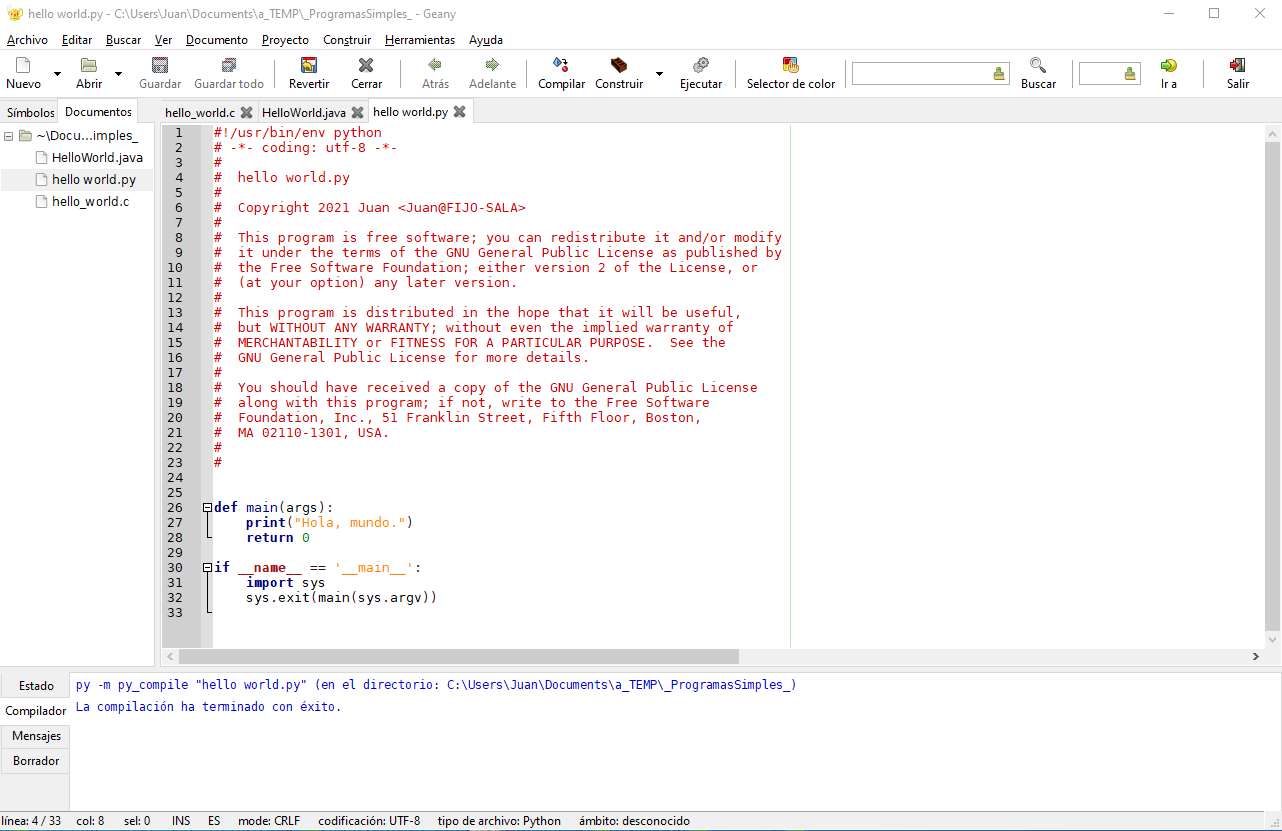
\includegraphics[width=0.95\textwidth]{pantallazo de Geany.png}


\subsection{BlueJ}

\url{https://www.bluej.org/}

Permite trabajar con Java. 

Como se ha comentado antes, el instalador de BlueJ instala también las herramientas de desarrollo Java JDK. Es un ``todo en uno'' muy sencillo de instalar.

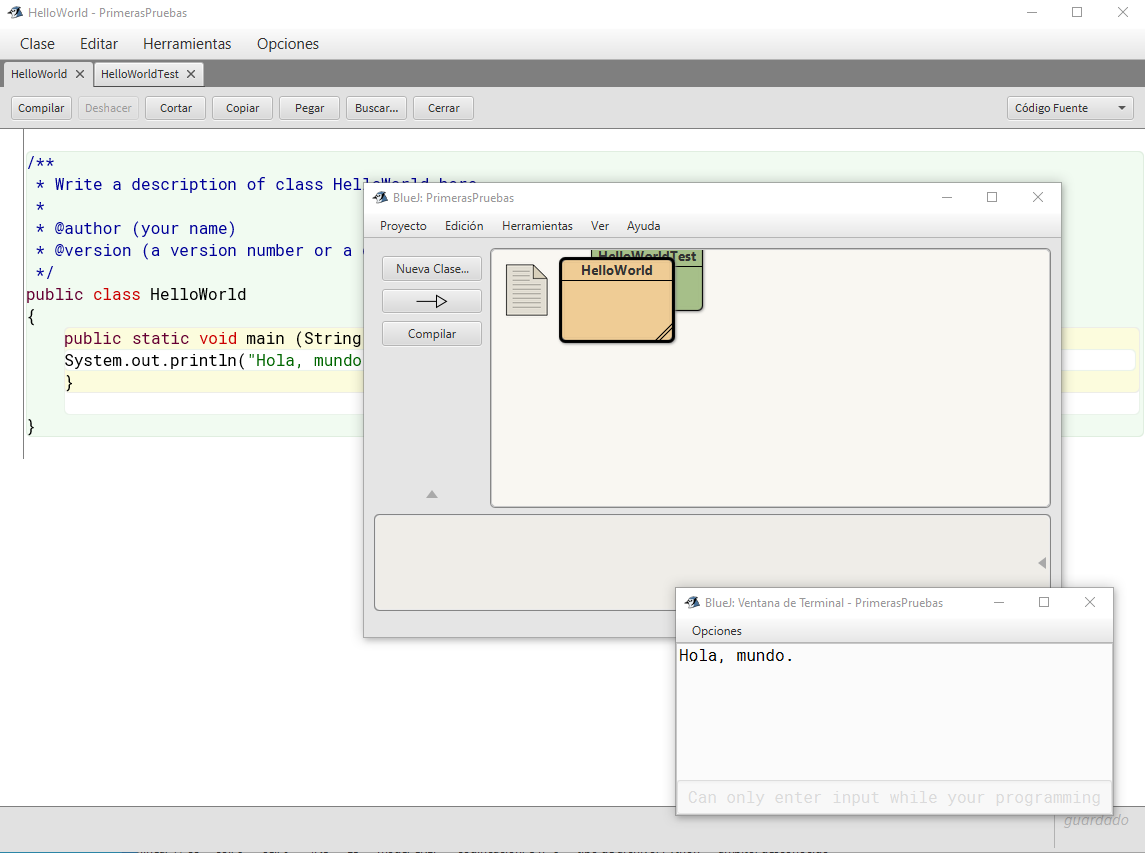
\includegraphics[width=0.8\textwidth]{pantallazo de BlueJ.png}


\subsection{Jet Brains edu}

Para trabajar con Pyton: \url{https://www.jetbrains.com/edu-products/download/#section=pycharm-edu}

Para trabajar con Java: \url{https://www.jetbrains.com/edu-products/download/#section=idea}

Las herramientas citadas son versiones educativas, para aprender; pero similares a las profesionales.

Si luego se van a realizar trabajos más serios, esta empresa cuenta con multitud de herramientas profesionales. \url{https://www.jetbrains.com/}

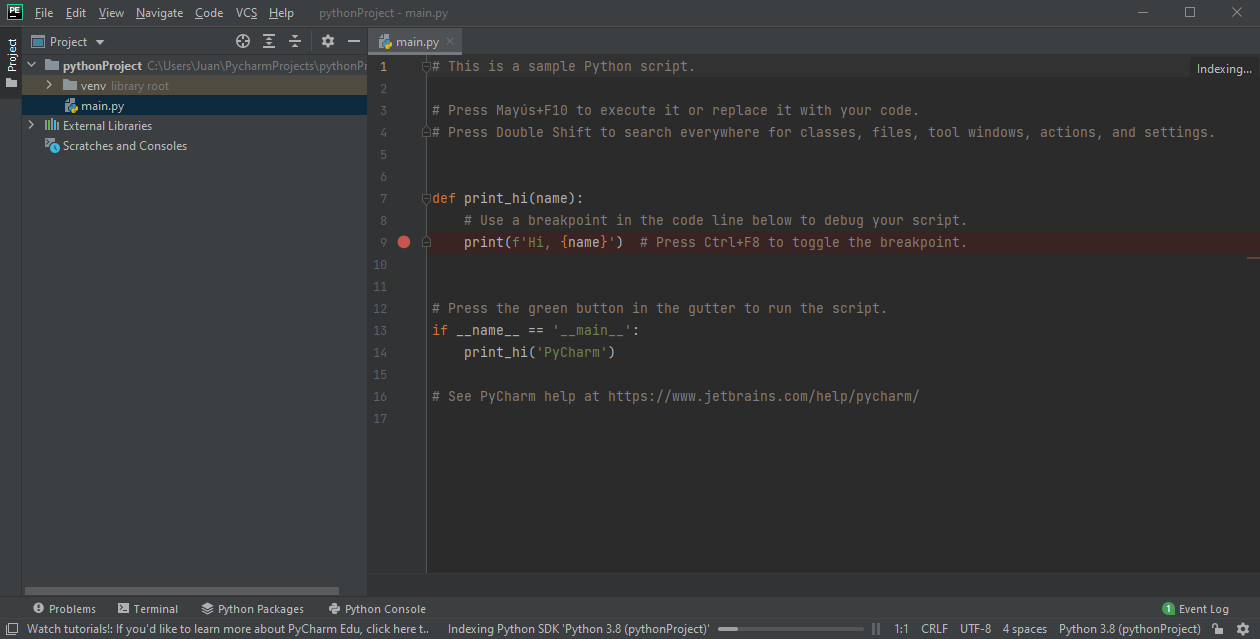
\includegraphics[width=0.85\textwidth]{pantallazo de PyCharm.png}


\subsection{Visual Studio Code}

\url{https://code.visualstudio.com/}
\\ \url{https://code.visualstudio.com/docs}

Entre otros lenguajes, permite trabajar con Python, C/C++, C\# o Java.

nota: No confundir Visual Studio Code con su ``hermano mayor'' Visual Studio (\url{https://visualstudio.microsoft.com/vs/}), que es otro IDE completamente diferente,un IDE para uso profesional. Aunque tiene también una licencia ``Comunity'' gratuita.

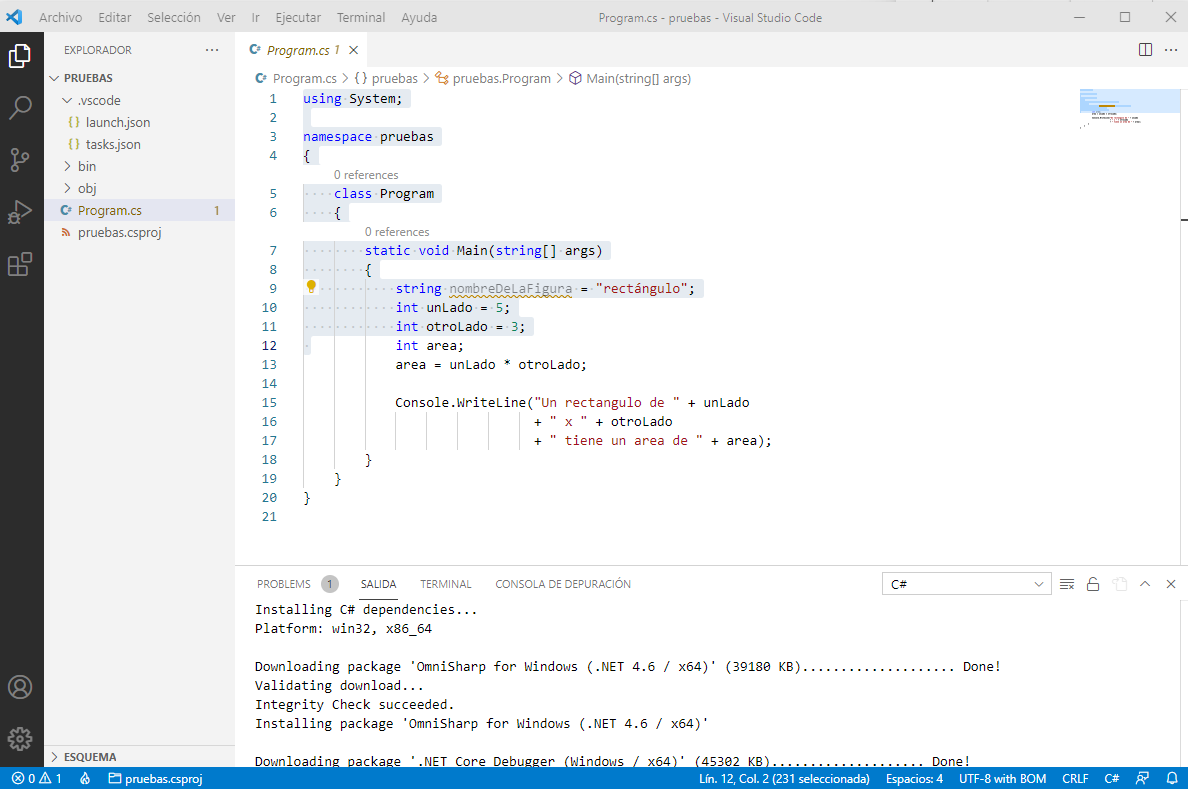
\includegraphics[width=\textwidth]{pantallazo de VSCode.png}


\section{Manos a la obra (3): comentarios y consejos varios}\label{manos_a_la_obra_3}

\subsection{Algunas peculiaridades de la sintaxis de Python}

La mayoría de lenguajes de programación suelen marcar los límites de sus estructuras con alguna marca de inicio y de fin. La más habitual suelen ser las llaves:  $\{ \ldots \}$

Pero Pyton marca los límites con la indentación (espacio en blanco al principio de cada línea). Todas las lineas seguidas que empiezan en un mismo punto, forman un bloque. La primera línea que empiece en otro punto, ya no pertenece al bloque.

De esta manera, consigue que la indentación se respete siempre y que todos los programas tengan una apariencia similar. Facilitando mucho su lectura.

\begin{lstlisting}[frame=single, caption=lenguaje Python : indentación correcta]

import math

def main(args):

    esUnaCircunferencia = False
    print("Esto es por poner algo al principio...")

    if esUnaCircunferencia:
        radio = 5
        diametro = radio * 2
        area = 2 * math.pi * radio
        print(f"El area de un circulo",
              f"de radio {radio} es {area}")
    else:
        unLado = 7
        otroLado = 3
        area = unLado * otroLado
        print(f"El area de un cuadrado",
              f"de lados {unLado} x {otroLado}",
              f"es {area}")

    print("Esto es por poner algo al final...")

    return 0


if __name__ == '__main__':
    import sys
    sys.exit(main(sys.argv))
\end{lstlisting}

\begin{lstlisting}[frame=single, caption=lenguaje Java : indentación correcta]

public class indentacion_bien {
	
    public static void main (String[] args) {
        
        Boolean esUnaCircunferencia = false;
        System.out.println("Esto es por poner algo al principio...");
        
        if(esUnaCircunferencia) {
            Double radio = 5.0;
            Double diametro = radio * 2.0;
            Double area = 2.0 * Math.PI * radio;
            System.out.println("El area de un circulo de radio " + radio 
                               + " es " + area);
        }
        else {
            Double unLado = 7.0;
            Double otroLado = 3.0;
            Double area = unLado * otroLado;
            System.out.println("El area de un cuadrado de lados "
                               + unLado + " x " + otroLado 
                               + " es " + area);
        }
              
        System.out.println("Esto es por poner algo al final...");
        
    }
    
}
\end{lstlisting}


\begin{lstlisting}[frame=single, caption=lenguaje Java : indentación lo peor posible]

public class indentacionFatal {
public static void main (String[] args) {
Boolean esUnaCircunferencia = false;
System.out.println("Esto funciona igual de bien que antes...");
if(esUnaCircunferencia) {
Double radio = 5.0;
Double diametro = radio * 2.0;
Double area = 2.0 * Math.PI * radio;
System.out.println("El area de un circulo de radio " + radio 
+ " es " + area);
}
else {
Double unLado = 7.0;
Double otroLado = 3.0;
Double area = unLado * otroLado;
System.out.println("El area de un cuadrado de lados "
+ unLado + " x " + otroLado 
+ " es " + area);
}
System.out.println("Pero es mas dificil de leer...");
}
}
\end{lstlisting}


\begin{lstlisting}[frame=single, caption=lenguaje Python : indentación lo peor posible]

import math
def main(args):
 esUnaCircunferencia = False
 print("Esto es por poner algo al principio...")
 if esUnaCircunferencia:
  radio = 5
  diametro = radio * 2
  area = 2 * math.pi * radio
  print(f"El area de un circulo",
   f"de radio {radio} es {area}")
 else:
  unLado = 7
  otroLado = 3
  area = unLado * otroLado
  print(f"El area de un cuadrado",
   f"de lados {unLado} x {otroLado}",
   f"es {area}")
 print("Esto es por poner algo al final...")
 return 0
if __name__ == '__main__':
 import sys
 sys.exit(main(sys.argv))
\end{lstlisting}


\subsection{El gestor de paquetes de Python}

El lenguage Python tiene un gestor de paquetes (bibliotecas de funciones). Antes de utilizar uno de esos paquetes en nuestros programas (import), es necesario tenerlo instalado en nuestro entorno de programación. La herramienta para hacerlo es \textbf{pip}. Esta herramienta se ejecuta  abriendo una ventana de sistema y escribiendo el comando con su parámetro `install' más el nombre del paquete a instalar. Por ejemplo:
\begin{lstlisting}
PS C:\Users\Juan> pip install numpy
Collecting numpy
  Downloading numpy-1.20.3-cp38-cp38-win_amd64.whl (13.7 MB)
Installing collected packages: numpy
Successfully installed numpy-1.20.3

PS C:\Users\Juan> pip install matplotlib
Collecting matplotlib
  Downloading matplotlib-3.4.2-cp38-cp38-win_amd64.whl (7.1 MB)
Requirement already satisfied: numpy>=1.16 in c:\users\juan\appdata\local\programs\python\python38\lib\site-packages (from matplotlib) (1.20.3)
Requirement already satisfied: pyparsing>=2.2.1 in c:\users\juan\appdata\local\programs\python\python38\lib\site-packages (from matplotlib) (2.4.7)
Collecting cycler>=0.10
  Downloading cycler-0.10.0-py2.py3-none-any.whl (6.5 kB)
Collecting pillow>=6.2.0
  Downloading Pillow-8.2.0-cp38-cp38-win_amd64.whl (2.2 MB)
Collecting kiwisolver>=1.0.1
  Downloading kiwisolver-1.3.1-cp38-cp38-win_amd64.whl (51 kB)
Requirement already satisfied: python-dateutil>=2.7 in c:\users\juan\appdata\local\programs\python\python38\lib\site-packages (from matplotlib) (2.8.1)
Requirement already satisfied: six in c:\users\juan\appdata\local\programs\python\python38\lib\site-packages (from cycler>=0.10->matplotlib) (1.15.0)
Installing collected packages: cycler, pillow, kiwisolver, matplotlib
Successfully installed cycler-0.10.0 kiwisolver-1.3.1 matplotlib-3.4.2 pillow-8.2.0
\end{lstlisting}

nota: En el ejemplo precedente se han instalado estos dos paquetes:
\begin{itemize}
\item numpy: \url{https://pypi.org/project/numpy/}
\item matplotlib: \url{https://pypi.org/project/matplotlib/}
\\{\footnotesize nota: este paquete depende a su vez de otros paquetes: numpy, pyparsing, cycler, pillow, kiwisolver, python-dateutil y six, que también han sido instalados si es que no estaban ya instalados con anterioridad.}
\end{itemize}


\subsection{Uso del IDE Geany}

Para empezar un nuevo programa, usar la plantilla correspondiente al lenguaje deseado:

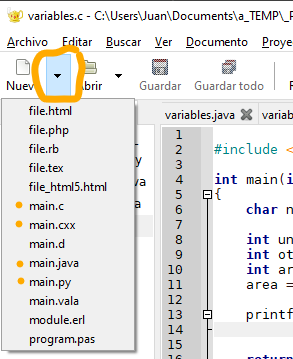
\includegraphics[width=0.45\textwidth]{Geany - nuevo - barra}
\hspace{0.1\textwidth}
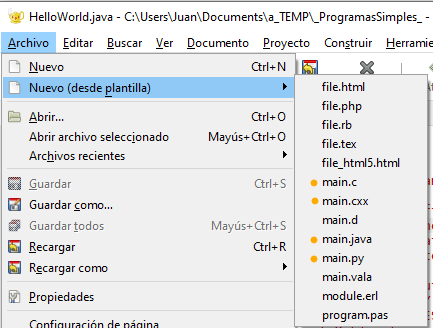
\includegraphics[width=0.45\textwidth]{Geany - nuevo - menu}

Para ejecutar el programa:
\begin{itemize}
\item Si es Python, con `Ejecutar' es suficiente; ya que Python es un lenguaje interpretado.
\item Si es Java, primero se ha de `Compilar' y luego, una vez compilado, ya se puede `Ejecutar'.
\item Si es C o C++, primero se ha de `Compilar', luego se ha de `Construir' (linkar) y luego, una vez construido, ya se puede `Ejecutar'.
\end{itemize}
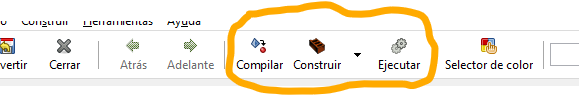
\includegraphics[width=\textwidth]{Geany - compilar y ejecutar - barra}

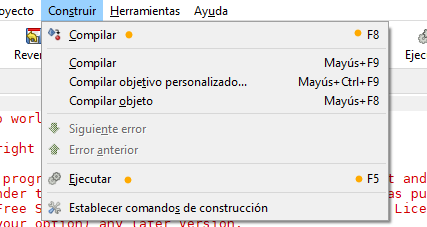
\includegraphics[width=0.45\textwidth]{Geany - compilar y ejecutar - menu}


\subsection{Uso del IDE Visual Studio Code}

Para cambiar el idioma del entorno, ir al menú `View' `Command Palette' (`Ver' `Paleta de comandos') y comenzar a teclear la palabra language . Aparecerá la opción `Configure display language' (`Seleccionar idioma para mostrar'), que permite instalar nuevos idiomas (`Install Additional Languages'). Una vez instalado, repitiendo el proceso se podrá escoger como idioma de trabajo; y reiniciando (restart) quedara activado.
\\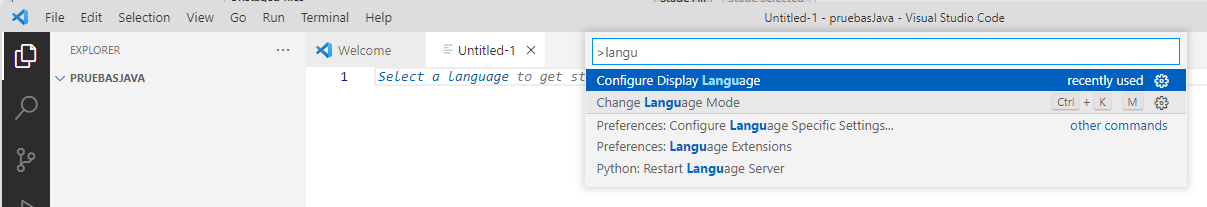
\includegraphics[width=\textwidth]{VScode - choose language}
\\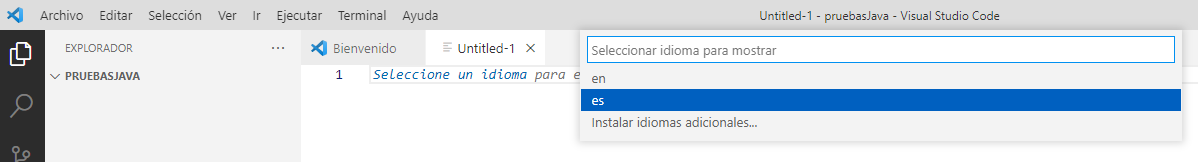
\includegraphics[width=\textwidth]{VScode - elegir idioma}

\vspace{0.5cm}
Para trabajar con alguno de los lenguajes de programación soportados por el entorno, se ha de instalar primero la extensión o extensiones apropiadas.
\\ \url{https://code.visualstudio.com/docs/languages/overview}
\\Ir al menú `View' `Extensions' (`Ver' `Extensiones') y teclear el nombre del lenguaje deseado.
\\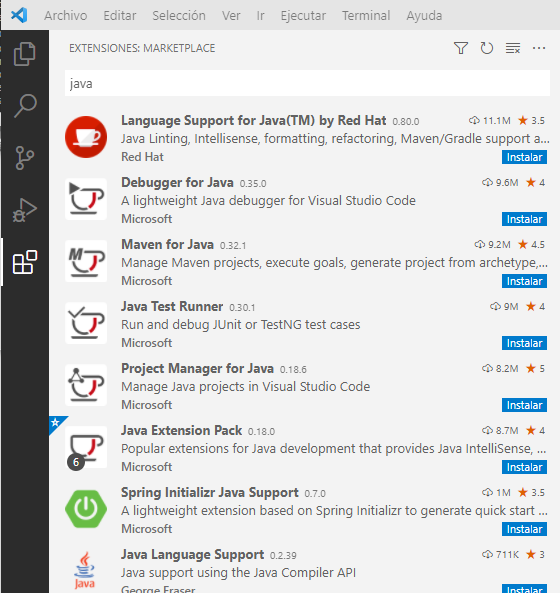
\includegraphics[scale=0.4]{VScode - instalar extensiones}
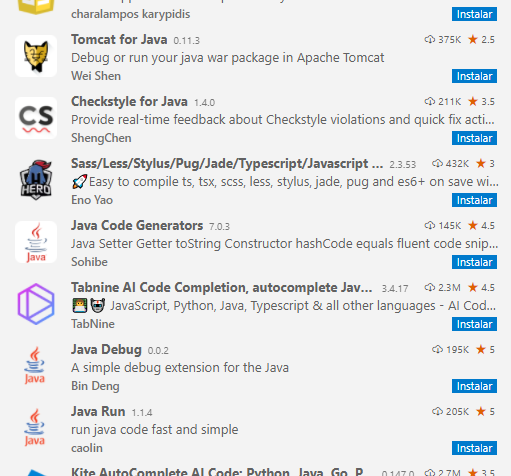
\includegraphics[scale=0.4]{VScode - instalar extensiones II}

\vspace{0.5cm}
Para iniciar un nuevo proyecto:
\begin{enumerate}
\item Abrir una carpeta donde agrupar los archivos del proyecto, con el menú `File' `Open Folder' (`Archivo' `Abrir Carpeta'). Creando antes la carpeta si es necesario.
\item Abrir la terminal con el menú `View' `Terminal' (`Ver' `Terminal') y teclear el comando pertinente. Por ejemplo:
\begin{itemize}
\item Un proyecto de aplicación .NET con interfaz de línea de comandos: \\ \verb!dotnet new console -o nombredelproyecto!
\item Un proyecto de aplicación .NET con interfaz gráfico Forms: \\ \verb!dotnet new winforms -o nombredelproyecto!
\item Un proyecto de biblioteca DLL: \\ \verb!dotnet new classlib -o nombredelproyecto!
\item etc.
\end{itemize} 
nota: una lista completa de todos los tipos de proyecto .NET se obtiene con el comando \verb!dotnet new --list!
\end{enumerate}


\section{Enlaces a referencias sobre la sintaxis de los lenguajes y sus bibliotecas base}


\subsection{referencias Python}

La referencia oficial sobre el lenguaje de programación Python está en:
\\ \url{https://docs.python.org/3/reference}
\\ \url{https://docs.python.org/3/library}
\\ \url{https://docs.python.org/3/tutorial}

Las personas que programan en Python suelen seguir ciertas normas de estilo para garantizar la legibilidad de sus programas:
\\ \url{https://www.python.org/dev/peps/pep-0008/}
\\ \url{https://docs.python-guide.org/writing/style/}



\subsection{referencias Java}

La referencia oficial sobre lenguaje de programación Java está en:
\\ \url{https://docs.oracle.com/javase/specs/jls/se16/html/index.html}
\\ \url{https://docs.oracle.com/en/java/javase/16/core/java-core-libraries1.html}
\\ \url{https://docs.oracle.com/en/java/javase/16/docs/api/index.html}
\\ \url{https://docs.oracle.com/javase/tutorial/tutorialLearningPaths.html}



\subsection{referencias C\#}

La referencia oficial sobre el lenguaje de programación C\# está en:
\\ \url{https://docs.microsoft.com/es-es/dotnet/csharp/language-reference/}
\\ \url{https://docs.microsoft.com/es-es/dotnet/api/?view=net-5.0}
\\ \url{https://docs.microsoft.com/es-es/dotnet/api/?view=netframework-4.8}
\\ \url{https://docs.microsoft.com/es-es/dotnet/standard/get-started}




\subsection{referencias C o C++}

La referencia oficial sobre el lenguaje de programación C es el libro:
\\ ``El lenguaje de Progamación C''. Brian Kernighan and Dennis Ritchie.

La referencia oficial sobre el lenguaje de programación C++ es el libro:
\\ ``El Lenguaje de Programación C++''. Bjarne Stroustrup.

Un par de sitios de referencia sobre el lenguaje de programación C:
\\ \url{https://en.cppreference.com/w/c/language}
\\ \url{https://en.cppreference.com/w/c}
\\ \url{http://www.cplusplus.com/reference/clibrary/}

Un par de sitios de referencia sobre el lenguaje de programación C++:
\\ \url{https://en.cppreference.com/w/cpp/language}
\\ \url{https://en.cppreference.com/w/cpp}
\\ \url{http://www.cplusplus.com/reference/}
\\ \url{http://www.cplusplus.com/doc/tutorial/}




\section{Enlaces a referencias sobre bibliotecas de funciones} \label{referencias_de_bibliotecas} 

\begin{itemize}

\item Por un lado, están las bibliotecas estándares del lenguaje de programación en que trabajemos:

\begin{itemize}

\item lenguaje Python
\\ \url{https://docs.python.org/3/library/}

\item lenguaje Java
\\ \url{https://docs.oracle.com/en/java/javase/17/docs/api/index.html}

\item lenguaje C\#
\\ \url{https://docs.microsoft.com/es-es/dotnet/api/?view=net-6.0}

\item lenguaje C o C++
\\ \url{http://www.cplusplus.com/reference/}
\\ \url{https://en.cppreference.com/w/}

\end{itemize}

\item Por otro lado, están las bibliotecas que podemos encontrar a través de Internet, en repositorios tales como
\\ \url{https://github.com/} 
\\ \url{https://pypi.org/search/} 
\\ \url{https://mvnrepository.com/open-source} 
\\ \url{https://www.nuget.org/packages} 
\\ \url{https://packages.debian.org/stable/libs/} 
\\ \url{https://conan.io/center/} 
etc.

Algunas de estas bibliotecas son libres y otras suelen ser comerciales. Es importante leer con detenimiento las cláusulas de licencia que acompañan a cada una de ellas, para saber en qué condiciones las podemos utilizar en nuestros programas.

Antaño, utilizar una biblioteca requería conocer unos cuantos procesos bastante manuales. Hoy en día, es cada vez más frecuente disponer de gestores de paquetes integrados en el propio entorno de desarrollo. Estos gestores facilitan mucho la búsqueda de bibliotecas, su descarga e integración en el programa que se está desarrollando.
\\Algunos ejemplos:
\\ \url{https://es.wikipedia.org/wiki/Pip_(administrador_de_paquetes)}
\\ \url{https://es.wikipedia.org/wiki/Maven}
\\ \url{https://en.wikipedia.org/wiki/NuGet}
\\ \url{https://conan.io/}


\item Y para completar el tema, comentar que algunos programas de aplicación de usuario suelen disponer de una especie de ``biblioteca'' denominada API (Application Programming Interface). Pensada para poder interactuar con ellos desde otros programas externos y permitir programar complementos (add-ins). Por ejemplo:
\\ Revit API
\\ \url{https://www.revitapidocs.com/2022/}
\\ PyRevit
\\ \url{https://github.com/eirannejad/pyRevit}
\\ Archicad API
\\ \url{https://archicadapi.graphisoft.com/documentation/function-reference}
\\ PythonParts - Allplan
\\ \url{https://www.allplan.com/pythonparts/}
\\ SDK - Vectorworks Developer \\ \url{http://developer.vectorworks.net/index.php/SDK}
\\ Complementos de Microsoft Office (Word, Excel, Powerpoint,\ldots)
\\ \url{https://docs.microsoft.com/es-es/office/dev/add-ins/overview/office-add-ins}

\end{itemize}


Aún a costa de parecer pesado, insisto en lo comentado en el capítulo \ref{la_importancia_de_las_bibliotecas}:

\begin{itemize}

\item Conociendo las bibliotecas existentes evitaremos ``reinventar la rueda'' continuamente o, peor, quedarnos estancados en formas de programar anticuadas o ineficientes. 

\item Cuando nos enfrentamos por primera vez a una funcionalidad concreta. Es muy posible que otras personas la hayan tenido que implementar antes que nosotros. Y algunas puede que hayan tenido la delicadeza de plasmar su solución en una biblioteca reutilizable.

\item Cuando volvemos a enfrentamos a una funcionalidad concreta al cabo de unos cuantos años. Es muy posible que existan nuevas bibliotecas que aprovechen mejor las prestaciones de los ordenadores del momento.

\end{itemize}





\end{document}
